%
% ======================================================================
\RequirePackage{docswitch}
% \flag is set by the user, through the makefile:
%    make note
%    make apj
% etc.
\setjournal{\flag}

%\documentclass[\docopts]{\docclass}

% You could also define the document class directly
\documentclass[twocolumn]{aastex62}
% Custom commands from LSST DESC, see texmf/styles/lsstdesc_macros.sty
\usepackage{lsstdesc_macros}
\usepackage{tikz}
\usetikzlibrary{calc}
\usepackage{mwe}
\usepackage{graphicx}
\graphicspath{{./}{./figures/}}
\bibliographystyle{aj}
\extrafloats{100}
\usepackage{hyperref}
% Add your own macros here:
%\newcommand{\arcmin}{\unit{arcmin}}
%\newcommand{\arcsec}{\unit{arcsec}}
\newcommand{\rachel}[1]{{\textcolor{cyan}{{\textbf (RM: #1)}}}}


%
% ======================================================================

\begin{document}

\title[LSST DESC DC1]{The LSST DESC Data Challenge 1: Generation and Analysis of Synthetic Images for Next Generation Surveys }

%\maketitlepre

\begin{abstract}

The success of the Large Synoptic Survey Telescope (LSST) as a dark energy experiment will depend on controlling systematic biases in cosmological probes. Simulations are critical for developing the methodology to estimate and mitigate these systematics. In the first Data Challenge from the LSST Dark Energy Science Collaboration, we evaluate potential systematic biases in observables, with an emphasis on galaxy clustering. We simulate LSST images, then process and analyze them using the current version of the LSST Data Management pipeline. Then we characterize the resulting systematics and implement corrections. We also show that dithering reduces the impact of potential systematic effects. Our results demonstrate that we can generate realistic LSST-like simulated images and control the systematic effects, after processing these images, at a sufficient level to enable major advances in our knowledge of dark energy and cosmology. The methodology presented here can be easily translated to current and future imaging surveys.
\end{abstract}

% Keywords are ignored in the LSST DESC Note style:
\dockeys{large-scale structure of the universe}

%\maketitlepost

%\maketitle
% ----------------------------------------------------------------------
%

\section{Introduction}
\label{sec:intro}

\rachel{Should enlarge font in tick and axis labels to be comparable to font size in the paper
  text in all of the following figures: 4, 5, 6, 7, 8, 9, 11, 12, 13, 18, 19, 20.}

The increase in statistical power from recent cosmological experiments makes the modeling and mitigation of systematic uncertainties key to extracting the maximum amount of information from these surveys. More traditional in high energy particle physics~\citep{Brun:118715, 2006JHEP...05..026S}, end-to-end simulations provide a unique framework to
model systematics and streamline processing and analysis pipelines given out complete understanding of the inputs and outputs. With the increasing availability of computational resources, this approach has also been extended to photometric redshift galaxy surveys~\citep{2016MNRAS.457..786S,2016ApJ...817...25B} \rachel{We should rethink how we frame this.  First, DES is not just a photometric redshift survey -- let's call it an imaging survey.  Second, Balrog is not actually an end-to-end {\em ab initio} simulation tool as is implied here.  So we need to either make the text a little more nuanced and refer to the concept of injection simulations, or remove the Suchyta ref.}, and similar efforts are seen in spectroscopic surveys such as DESI~\citep{2016arXiv161100036D}.

For surveys like the LSST~\citep{Overview}, where the expected data volume is very large, and where a highly stringent control of the systematic uncertainties is required, producing these
kind of end-to-end simulations enables successful validation and verification of the processing and analysis pipelines. With $\sim 50$ PB of raw data and $\sim 40$ billion objects~\citep{Overview} the data handling by itself becomes challenging. \rachel{Those numbers are a bit deceptive, because they are for the entire LSST survey, right?  Whereas I think the point that's more relevant is that even simulations of a small subset of the LSST area, as we are doing here, comes with challenges.} There are many approaches to generate these end-to-end simulations. Usually, one would start from a source catalog where the objects are modeled according to certain parameters (sizes, shapes, fluxes), then render images from these sources, add some observational effects and, finally, use a software of choice to detect and measure the different properties of these images. Depending on the approach used to generate these images, some difficulties may arise when trying to relate inputs and outputs, especially in a very deep survey like LSST.

In this paper, we present and use simulated images that resemble the data that will be produced by
LSST~\citep{Overview} after 10 years of operation in $r$-band using state of the art tools produced by DESC and LSST. \rachel{Mention area difference?} We characterize the products of this process, measuring photometric, astrometric and clustering properties of the sample. These products encompass single-visit and coadded calibrated exposures (i.e., flattened, background subtracted, etc.) and source catalogs that take up to $\sim 225$ TB of disk space. We perform the 2-point clustering analysis in real and harmonic space for these simulations and assess the impact of potential systematics.

\textcolor{red}{MORE INTRODUCTION!!!}
\rachel{Big picture suggestion: It might make sense to slightly reframe this in a way that introduces the entire series of DESC data challenges DC1--DC3 as a way of ramping up in scope and complexity to LSST data, both to make increasingly sophisticated tests of analysis pipelines and to build up in the challenge for data processing/storage/serving.  This might involve some additional text plus changes in the narrative.  If you think this is worthwhile, I'm happy to take a stab at it, just let me know.}

This paper is structured as follows: In \secref{inputs}, we describe the inputs for our simulated images. In \secref{dithering}, we discuss the dither strategies used for this study. In \secref{image_generation_pipeline}, we describe the process used to generate LSST-like artificial images. In \secref{catalogs}, we describe the processed data products generated and perform several validation tests. In \secref{analysis}, we present the clustering analyses on the simulated data products. Finally, in \secref{conclusions}, we present some concluding remarks.

\rachel{Big picture suggestion: The paper structure might be easier for people to follow if we have some kind of high-level flowchart showing what are the steps in producing and analyzing the simulations, and how they map onto paper sections.  I also feel that we are missing an entire section on the factors that drove the simulation design: why did we design it this way?  Currently the design is described in an almost offhand way in the end of section 2 (and a bit in the end of section 3), where it doesn't fit thematically, and no rationale is given.  A bit of the design philosophy is also given in section 4.1, but even there it's incomplete.  So perhaps we could insert a section at this point on the simulation design and workflow, which would explain the factors underlying the DC1 design and provide the flowchart for the various steps in the process?  This might follow nicely from the text that I proposed we add in the intro regarding DC1 in the context of the entire series of data challenges.}

%One of the most critical aspects in Stage IV experiments is the characterization of their instrumentation and systematic effects~\citep{2006astro.ph..9591A}. In the case of  LSST~\citep{2008arXiv0805.2366I,ScienceBook,WhitePaper} this becomes especially difficult given its wide variety of cosmological probes. In this paper we present a methodology to characterize the LSST large-scale structure (LSS) transfer function and an analysis of potential systematic effects present in LSS analyses. \CHECK{rewrite}
% ---------------------------------------------------------------------
\section{Image generation: input catalog}
\label{sec:inputs}
Image simulations allow us to study in detail the detection and deblending properties of a given image-processing pipeline. For example, if we produce images using an object catalog with random positions uniformly distributed across the sky, as well as uniformly random shapes and fluxes, we can get information about detection efficiencies as a function of flux.  However, the information about blending will not be realistic and we will not be able to capture some correlations present in real data. On the other hand, using N-body simulations as the input to generate artificial images allows us to study all the aforementioned effects. This is why we used the \texttt{CatSim}~\citep{2010SPIE.7738E..1OC,2014SPIE.9150E..14C} catalog as our input.  \texttt{CatSim} is a set of simulations provided by the LSST Simulations Team representing a realistic distribution of both Milky Way and extra-galactic sources.  The LSST Simulations webpage\footnote{\url{https://www.lsst.org/scientists/simulations/catsim}} describes the physical models underlying \texttt{CatSim} as follows:
\rachel{Does it really make sense to quote this extensively?  Perhaps we could paraphrase instead?}
\begin{quote}
[The extra-galactic catalog] uses the dark matter haloes from the Millennium simulation~\citep{2005Nature.435.629S} and a semi-analytic baryon model described in \citet{2006MNRAS.366..499D}. The semi-analytic model features radiative cooling, star formation, the dynamics of black holes, supernovae, and AGNs and was adjusted to mimic the luminosity, color, and morphology distributions of low redshift galaxies.  [\texttt{CatSim} was] generated by constructing a lightcone, covering redshifts $0<z<6$ from 58 500 $h^{-1}$ Mpc simulation snapshots. The final catalog comprises a 4.5$\times$4.5 degree footprint on the sky (sufficient to cover a single LSST field-of-view) and samples halo masses over the range $2.5\times10^{9}$ to $10^{12}$ $\Msun$.

...For all sources, a spectral energy distribution (SED), is fit to the galaxy colors using \citet{2003MNRAS.344.1000B} spectral synthesis models. The \citet{2006MNRAS.366..499D} catalog includes BVRIK magnitudes and dust values for the disk and bulge components of each galaxy as well as radii, redshift, coordinates, stellar age, masses and metallicities. Fits are undertaken independently for the bulge and disk and include inclination dependent reddening. Morphologies are modeled using two S\'{e}rsic profiles~\citep{1963BAAA....6...41S} and a single point source (for the AGN). Bulge-to-disk ratios and disk scale lengths are taken from \citep{2006MNRAS.366..499D}. Half-light radii for the bulge components are derived from the absolute-magnitude vs half-light radius relation given by \citet{2011A&A...534A...3G}. Colors and stellar mass of the AGN host galaxies are estimated from the AGN luminosities.

Stars are represented as point sources and are drawn from the Galfast model~\citep{2008ApJ...673..864J}. Galfast generates stars according to density laws derived from fitting SDSS data to a model of a thick and thin disk, and a halo. Each star is assigned a metallicity, proper motion, and parallax.
\end{quote}

For the Data Challenge 1 (DC1), the extra-galactic catalog was tiled to generate a $\sim 40$ deg$^{2}$ footprint. This approach introduces a periodicity that induces extra correlations in our sample, however, we confirmed that these effects appear at scales larger than we are able to map given the DC1 area.

In total \rachel{after tiling?}, the input catalog contains approximately $63.1$ million sources of which, $61.3$ million are galaxies whose redshift and magnitude distributions are depicted in \figref{catalog_plots} and $1.8$ million are stars. We simulate images in $r$-band to LSST full depth ($10$ years). The final footprint can be seen in \figref{footprint}.  We simulate observations within this footprint using the \texttt{minion\_1016}\footnote{\url{https://www.lsst.org/scientists/simulations/opsim/opsim-v335-benchmark-surveys}} simulated observing cadence generated with the LSST Operations Simulator (OpSim)~\citep{2014SPIE.9150E..15D}.

\begin{figure}
\centering
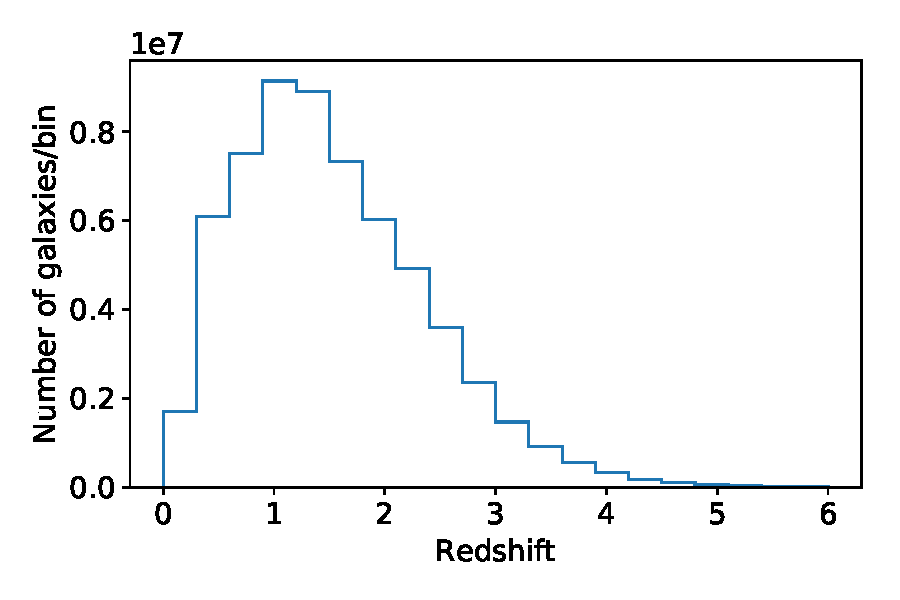
\includegraphics[width=0.9\columnwidth]{N_z_DC1.pdf}
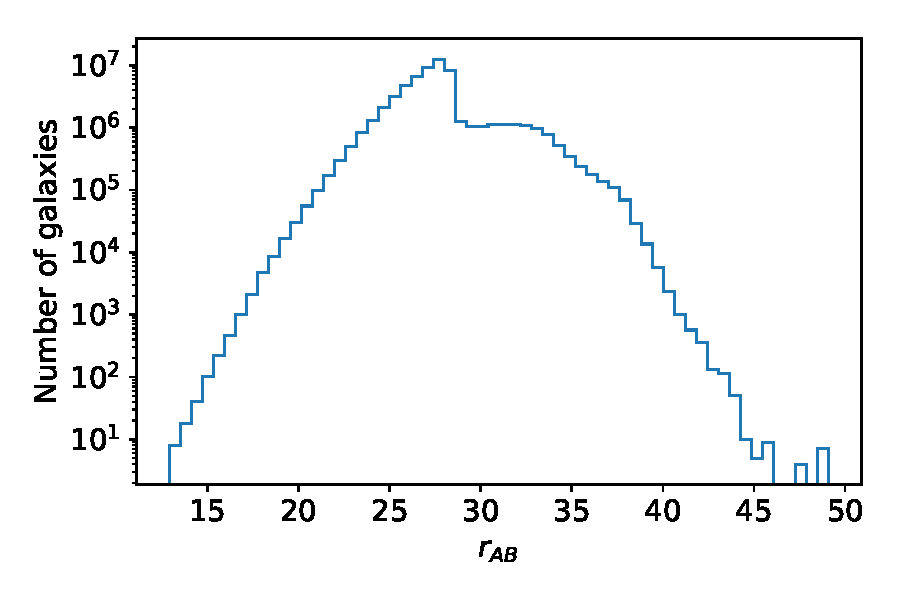
\includegraphics[width=0.9\columnwidth]{N_m_DC1.pdf}
\caption{Redshift (top) and magnitude (bottom) distribution for the galaxies used as inputs for DC1. \rachel{Does it really make sense to show anything beyond $r_{AB}\sim 30$?  Currently we spend half the plot there, but those objects are not relevant.  My suggestion: truncate at 30, and also put two vertical dashed lines, one corresponding to typical single-visit depth and one corresponding to the median coadded depth in the dithered case.}}
\label{fig:catalog_plots}
\end{figure}

\begin{figure}
\centering
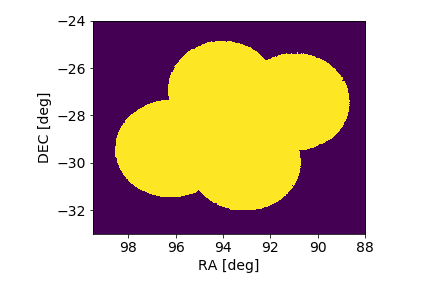
\includegraphics[width=0.9\columnwidth]{footprint.png}
\caption{Footprint of the DC1 dataset. We simulate 4 LSST full focal plane pointings which roughly corresponds to 40 deg$^{2}$.}
\label{fig:footprint}
\end{figure}

\section{Dither strategy}
\label{sec:dithering}

As mentioned earlier, we use OpSim's output, which contains a realization of the LSST observing cadence and the survey footprint. Since OpSim divides the sky with hexagonal tiles, the nominal telescope pointings lead to overlapping regions across adjacent tiles that are observed more often than the non-overlapping part of the field-of-view (FOV), resulting in depth non-uniformity on the scale of $\sim$1 degree and consequent systematic uncertainties \citep{2016ApJ...829...50A}. In an effort to mitigate these effects, we implement \textit{dithers} -- offsets in the nominal telescope pointings. Specifically, here we use \textit{large}, i.e., as large as the FOV, random translational dithers, implemented after every visit, and random rotational dithers implemented after every filter change. The specific translational dither strategy is chosen based on a more extensive study of the various (translational) dither strategies in \citet{2016ApJ...829...50A}, where random dithers after every visit are found to be amongst the most effective.

For our purposes, we consider both the undithered and the dithered observing strategy. For the dithered strategy, some visits will contain sensors that fall out of the DC1 region; these sensors were not simulated in order to save computational resources.

\section{Image generation: pipeline}
\label{sec:image_generation_pipeline}
% ---------------------------------------------------------------------

The artificial generation of astronomical images is a complex and computationally demanding process. In the recent
years, there have been major efforts in the community to create software that allows fast realistic image
simulation, such as \texttt{BALROG}~\citep{2016MNRAS.457..786S}, \texttt{UFIG}~\citep{2016ApJ...817...25B}, and \textsc{PhoSim}~\citep{2015ApJS..218...14P}. \rachel{Here too, I think that some changes are needed in the description.  Balrog is {\em not} an end-to-end simulation tool; UFIG is meant to be fast and not very realistic.  Perhaps reframe as ``\dots to create software that enables the generation of astronomical images, with various choices made in terms of level of complexity and fidelity, and computational efficiency, such as \dots''.} In our case, we model the input sources using imSim\footnote{\url{https://github.com/LSSTDESC/imSim}}, which uses \textsc{GalSim}~\citep{2015A&C....10..121R} as a library for image rendering, and uses LSST-specific information (e.g., about the geometry of the CCDs and the focal plane, the system throughputs in the different bands, etc.) to generate LSST-like images.

\subsection{imSim}
\label{sec:imsim_pipeline}

imSim is a fast image simulation software package that follows the path of similar efforts in the context of current imaging surveys~\citet{2016MNRAS.457..786S,2016ApJ...817...25B}.  \rachel{Here too, we should be careful: the design philosophy for those two codes is {\em entirely different} from imSim in my view.  One is for injection simulations only; the other is meant to be an ultra-fast image generation tool.  imSim uses GalSim with a modular approach, allowing one to dial up/down the level of fidelity of the simulations.} \rachel{For the sake of reproducibility, we need to say what imSim version was used, the fact that it is a pre-release (beta version), and that the text does not describe the current version of imSim.}

For DC1, we simulate each CCD of the focal plane individually, and instead of the planned two 15-seconds exposures~\citep{Overview}, we generate a single image with a 30-second exposure time to simplify the data handling. We omit instrumental effects and variability in the optical model across the focal plane. Since this is the first DESC data challenge, we want to ensure that we are able to generate and process the simplest cases, and then, build upon this base, increasing the complexity and level of realism for future data challenges. Our sky brightness model is based off the \citet{1991PASP..103.1033K} model provided by OpSim, refined by the detailed wavelength dependence of the phenomenological model from~\citet{2016SPIE.9910E..1AY}. The PSF model is a Gaussian for the system with a full-width half-maximum airmass dependence\footnote{From LSST-20160 eqn.~(4.1) \rachel{should link to this document / name it}} and a Kolmogorov profile to model the atmosphere which is also airmass dependent\footnote{From LSST-20160 eqn.~(4.2)}. \rachel{Can you explain why the system component is airmass dependent very briefly?  It's counter-intuitive, at least to me.} The airmass, $X$, depends on the angular distance to the zenith, $Z$, as follows~\citep{1991PASP..103.1033K}:
\begin{equation}
X = (1 - 0.96\sin{Z})^{-0.5}.
\end{equation}

\subsubsection{Source rendering}
\rachel{I'm not sure it makes sense to have a single subsubsection inside of a subsection.}

imSim can generate three different types of objects: stars, which are modeled as PSF-like objects; galaxies, which are modeled as composite (bulge plus disk) S\'{e}rsic profiles~\citep{1963BAAA....6...41S} using
the parameters given by CatSim; and AGNs which are also modeled as point sources and, for simplicity, without any variability. Future versions of imSim will have the ability to generate more complex galaxy morphologies. The brightness for these sources is computed using the magnitudes from CatSim, which are converted to counts using the latest version of the LSST throughputs\footnote{\url{https://github.com/lsst/throughputs}}. We clip the objects at magnitude 10 in order to improve the numerical performance. \rachel{What is meant by ``numerical performance'' here?  Should this be ``computational efficiency''?  Or was there some numerical rendering error for the bright objects?}

The final products of this pipeline are FITS images with information about the observing conditions. We generated more than 200,000 images in total (including both the \textit{dithered}, and \textit{undithered} fields). The average time to simulate each CCD is $\sim 4300$ seconds and the total production time is $\sim 270,000$ CPU-hours.

% ----------------------------------------------------------------------

%\subsection{PhoSim}
%\label{sec:phosim_pipeline}

%PhoSim is a complementary approach where we use the photon-shooting software \textsc{PhoSim} to create simulated images.
%\textcolor{red}{Describe PhoSim. PhoSim inputs and differences with imSim. What are we adding?}
% ----------------------------------------------------------------------
\subsection{Image processing pipeline}
\label{sec:image_processing_pipeline}

\rachel{The section title is ``Image Generation: Pipeline'' which seems distinct from ``Image processing'' (this subsection).  Perhaps the section title should be changed to ``Image generation and processing'' to better reflect the section contents?}

The outputs of these simulations are then processed using the LSST data management (DM) stack~\citep{Overview,ScienceBook,WhitePaper,2017arXiv170506766B,2015arXiv151207914J}. \rachel{For the sake of reproducibility, we need to say what version of the DM stack was used for the processing.} The DM stack is an open-source, high-performance data processing and analysis system intended for use in optical and infrared survey data. The code can be found at \url{dm.lsst.org} and \url{pipelines.lsst.io}. The raw, uncalibrated single exposures are used as inputs. The software performs the reduction, detection, deblending and measurement on individual visits. It then coadds the images to produce the ``Level 2'' \rachel{I believe they have now changed this terminology - we should probably update.} data products~\citep{2015arXiv151207914J}. Although the DM stack is still under development, most of the pieces already meet the science requirements \rachel{science requirements for LSST in the LSST SRD?  I don't think that's the case\dots how was that confirmed?  It's not true, for example, for the PSF models.  Same concern applies if you are referring to the DESC SRD.}. The DM stack provides calibrated images and source catalogs for the individual visits and coadds stored in \texttt{FITS} files. In total, we detect and measure $\sim 10.6$ million objects with position, flux and shape information. We activated optional extensions for the pipeline to include \texttt{CMODEL} fluxes (see \cite{2017arXiv170506766B} for more details) and \texttt{HSM} shapes~\citep{2003MNRAS.343..459H,2005MNRAS.361.1287M}.

An example coadd cutout is shown in \figref{coadd_example}.

\rachel{Big picture comment: we don't talk at all about any of the software that drove these things - workflows for the DM processing etc.  Is that sufficiently trivial that it doesn't need to be mentioned?}

\begin{figure}
\centering
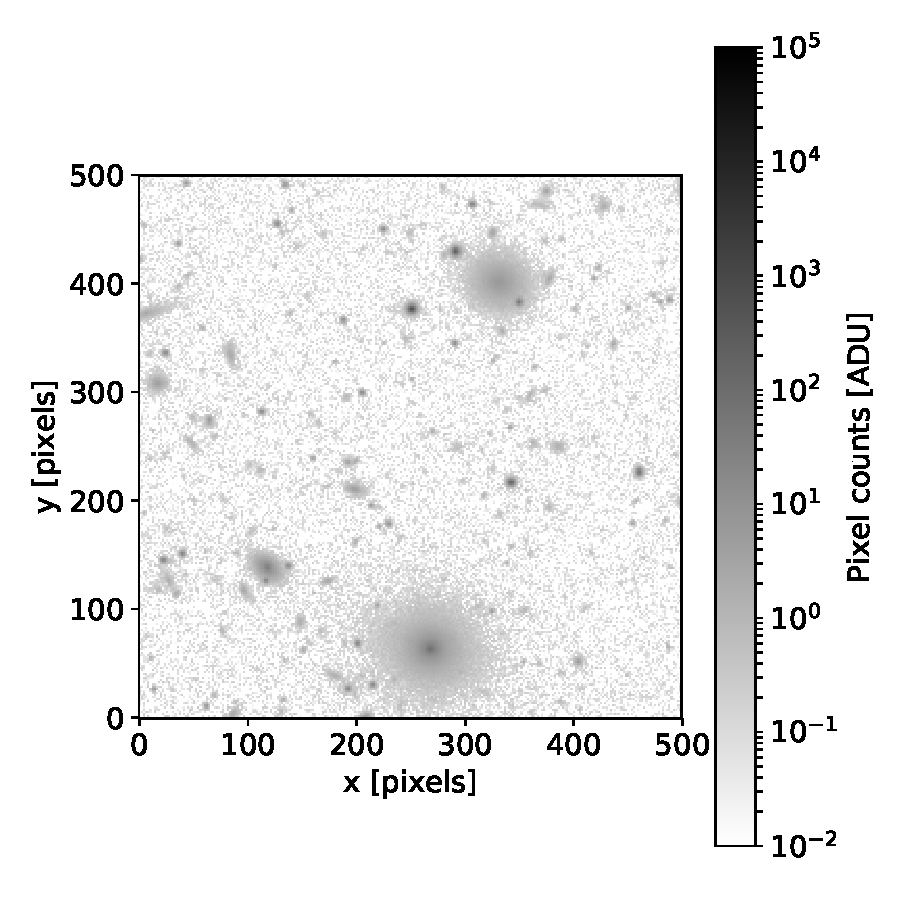
\includegraphics[width=0.9\columnwidth]{sample_coadd_DC1.pdf}
\caption{Example of a 500 $\times$ 500 pixel cutout from a full depth coadd showing the large density of objects in the LSST full-depth images.}
\label{fig:coadd_example}
\end{figure}

\section{Output catalogs and validation}
\label{sec:catalogs}

After being processed, the catalogs are stored at the National Energy Research Scientific Computing Center (NERSC)\footnote{\url{http://www.nersc.gov}} and accessible to DESC collaborators. We generate \texttt{pandas
dataframes}~\citep{mckinneypandas} and databases for each one of the coadds and input catalogs providing collaborators some flexibility in data access for their own analyses. As mentioned earlier, the output catalogs contain 10.6 million objects covering an area
of $\sim$ 43 deg$^{2}$. The catalogs include information about position, size, shape and magnitude for every object. They include several flags that give information about the presence of interpolated/saturated pixels in the objects and whether or not these objects are close to the edge of a CCD.

In order to check the level of realism and the accuracy of the processed catalogs we perform several quality assurance tests.

\subsection{Astrometry checks}
\label{sec:astrometry_checks}

Biases in astrometry can potentially affect both clustering and weak lensing measurements. We follow two approaches to check the quality of the astrometric solutions that we obtained: an \textit{external} check comparing to the input \textit{truth} catalog; and an \textit{internal} check comparing with different visits.

\subsubsection{External checks}
\label{sec:external_astrometry}

As we have already mentioned, one of the big advantages of using simulations is that we have access to the \textit{true} underlying information. We use this information to check the precision of the astrometric measurements in single exposures and coadds. We select stellar objects using the classifier included in the LSST software stack\footnote{To see more details about the classifier, refer to section 4.9.10 at ~\citet{2017arXiv170506766B}} and choose objects with \texttt{base\_ClassificationExtendedness\_value==0}.
We also require that \texttt{deblend\_nChild==0} to ensure that the objects are completely deblended, i.e., they are primary sources. We match these objects to the stellar sources in the input catalog. In both cases we use a \texttt{KDTree}~\citep{scikit-learn} to retrieve those objects in the input catalog that are within a 0.2 arc-seconds (one pixel) radius of those detected in the output catalog. We select the matched object that is closest in magnitude, only considering sources which have a magnitude difference smaller than 0.02 magnitudes. We discuss matching strategies in more detail at \secref{matching}.

We select a representative single visit (visit number $270675$ for the imSim dithered run) and calculate the difference between the measured and the input positions. These are represented in \figref{astrometry_a}. We see that both RA and Dec distributions are compatible with each other, indicating that there are no anisotropies in the detection.
However, we find that the distributions are asymmetric and that the median is not zero. This effect is even more noticeable in \figref{astrometry_b}, where we accumulated the results for 50 randomly selected visits of the imSim dithered simulation. This effect is also present in the undithered imSim run. This bias arises from the fact that the objects in the images include proper motion, which is unaccounted for in our \textit{truth tables}. However, this bias is below 15 mas, which is a much smaller scale than the resolution of the input N-body simulation. As a consequence we do not expect that the two point clustering statistics will be affected by this bias. We also checked the mean astrometric residual as a function of magnitude in \figref{astrometry_b}. We notice the same bias for the brightest objects (which are dominated by nearby sources), and so are the most affected by the effects of proper motion.

\begin{figure}
  \centering
  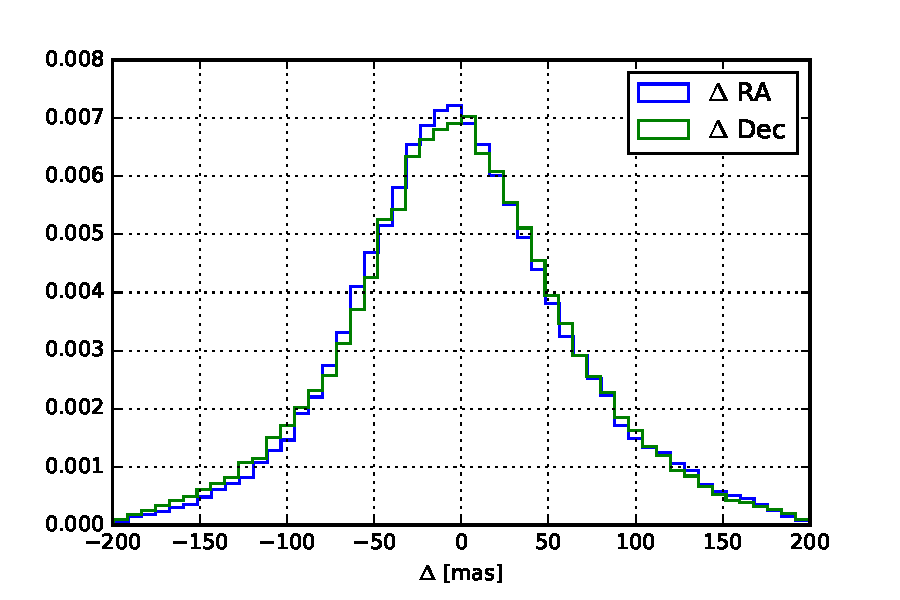
\includegraphics[width=0.45\textwidth]{astrometry_single_visit_imsim_dithered_hist}
  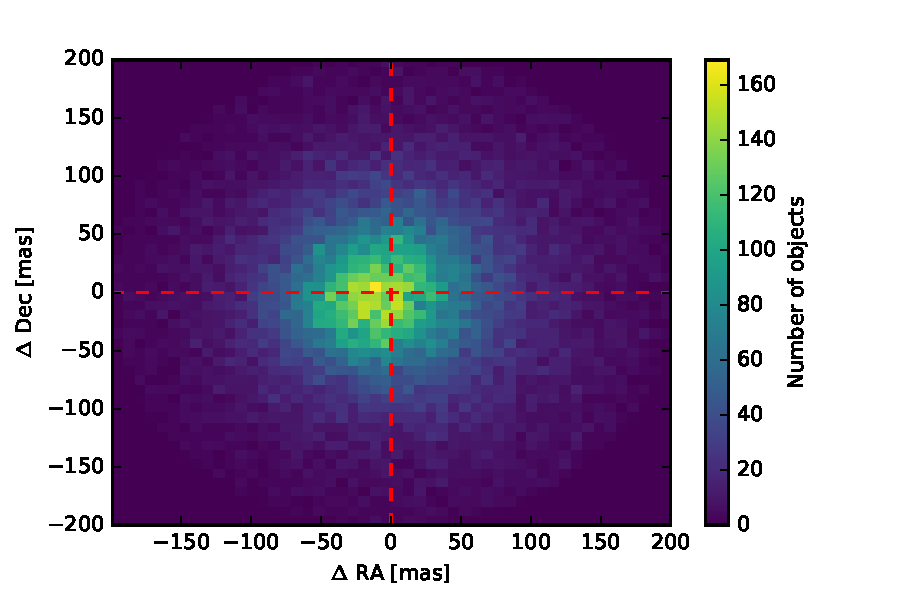
\includegraphics[width=0.45\textwidth]{astrometry_single_visit_imsim_dithered_hist2d}
  \caption{Top: Distribution of the difference $\Delta=X_{measured}-X_{input}$ in RA (blue) and Dec
    (green) coordinates for a randomly selected visit ($270675$ for the dithered run). We cannot see
    any differences between these. The histograms are normalized such that the total sum of the
    counts is equal to one. We measure a non-zero median, $\Delta_{median} \approx -2$ mas. Bottom:
    2D histogram showing the bivariate distribution of the difference in RA (horizontal axis) and
    Dec (vertical axis). The effect is similar for the undithered simulation. }
  \label{fig:astrometry_a}
\end{figure}

\begin{figure}
  \centering
  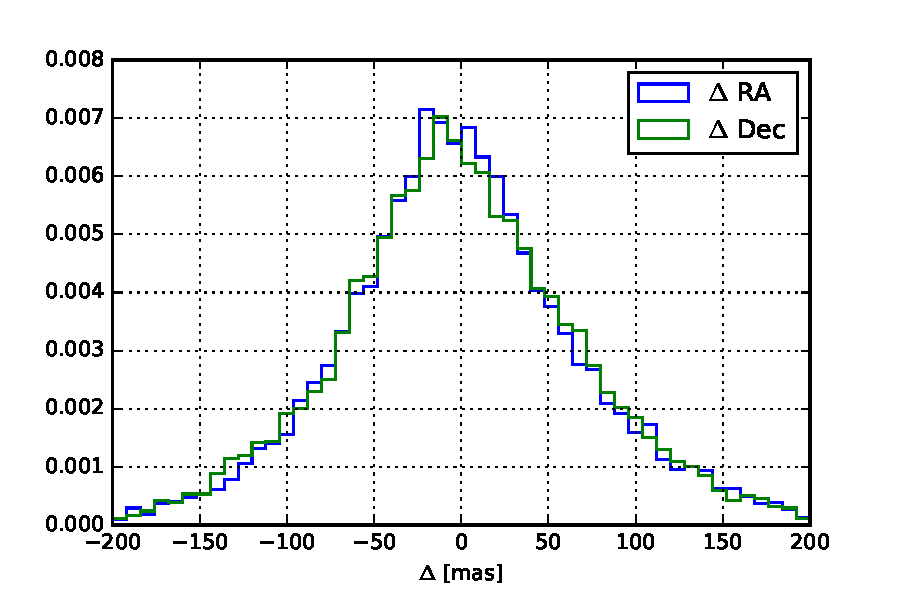
\includegraphics[width=0.45\textwidth]{astrometry_imsim_dithered_50visits}
  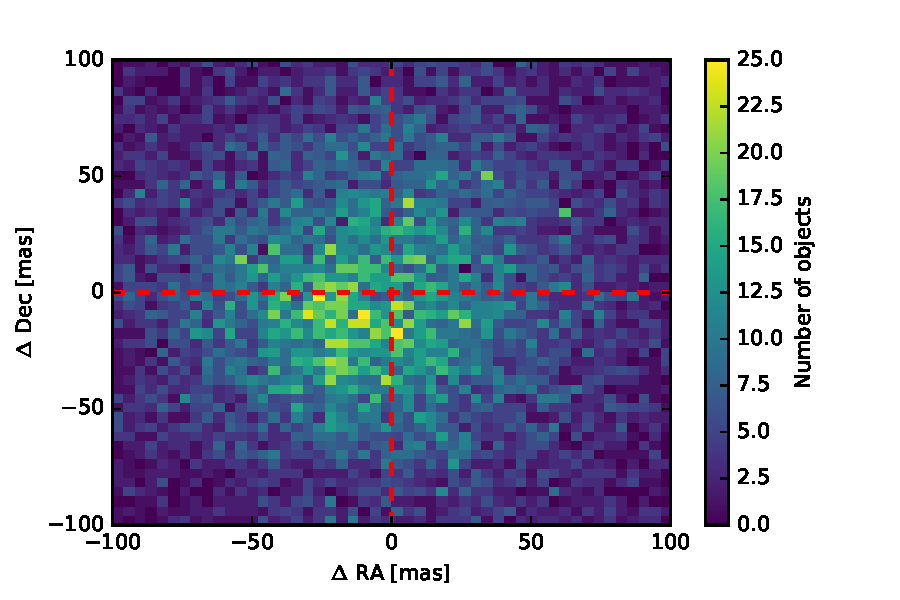
\includegraphics[width=0.45\textwidth]{astrometry_imsim_dithered_50visits_hist2d}
  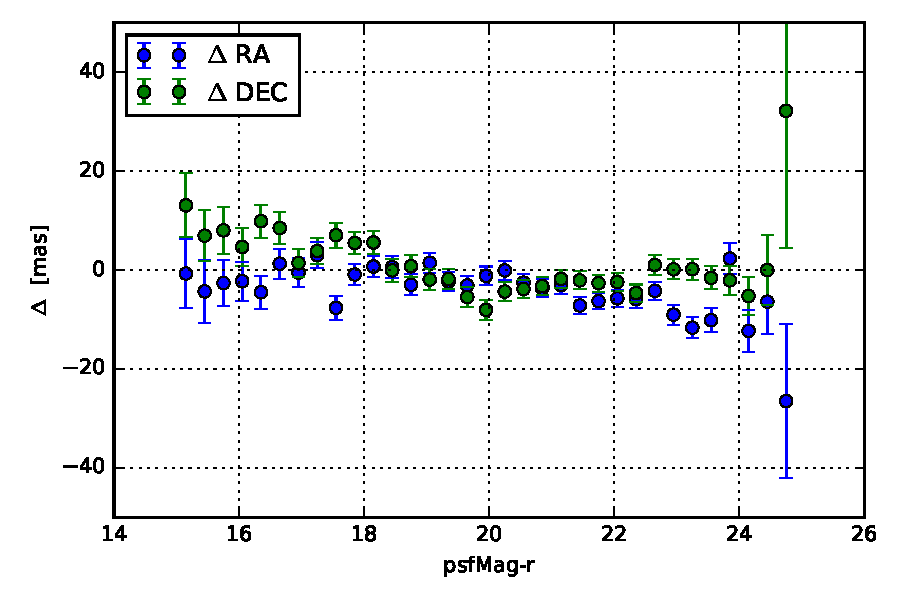
\includegraphics[width=0.45\textwidth]{astrometry_vs_mag_imsim_50_visits}
  \caption{Top: Distribution of the difference $\Delta=X_{measured}-X_{input}$ in RA (blue) and Dec (green) coordinates as in
  \figref{astrometry_a} but, accumulating the results for 50 randomly selected visits from the dithered run. Middle: 2D histogram
  showing the bivariate distribution of the difference in RA (horizontal axis) and Dec (vertical axis). Bottom: Mean astrometric residual
  as a function of magnitude for RA (blue) and Dec (green). These distributions are similar for the undithered run.}
  \label{fig:astrometry_b}
\end{figure}

In addition, we wanted to check if there is a preferred orientation for the differences between the input and output position in a single visit. Using the same visit as before, we show the astrometric residuals in \figref{astrometry_c}. We see that the astrometric residuals do not show any noticeable structure and appear to be mostly random with the largest contributions close to the CCD edges.

\begin{figure}
  \centering
  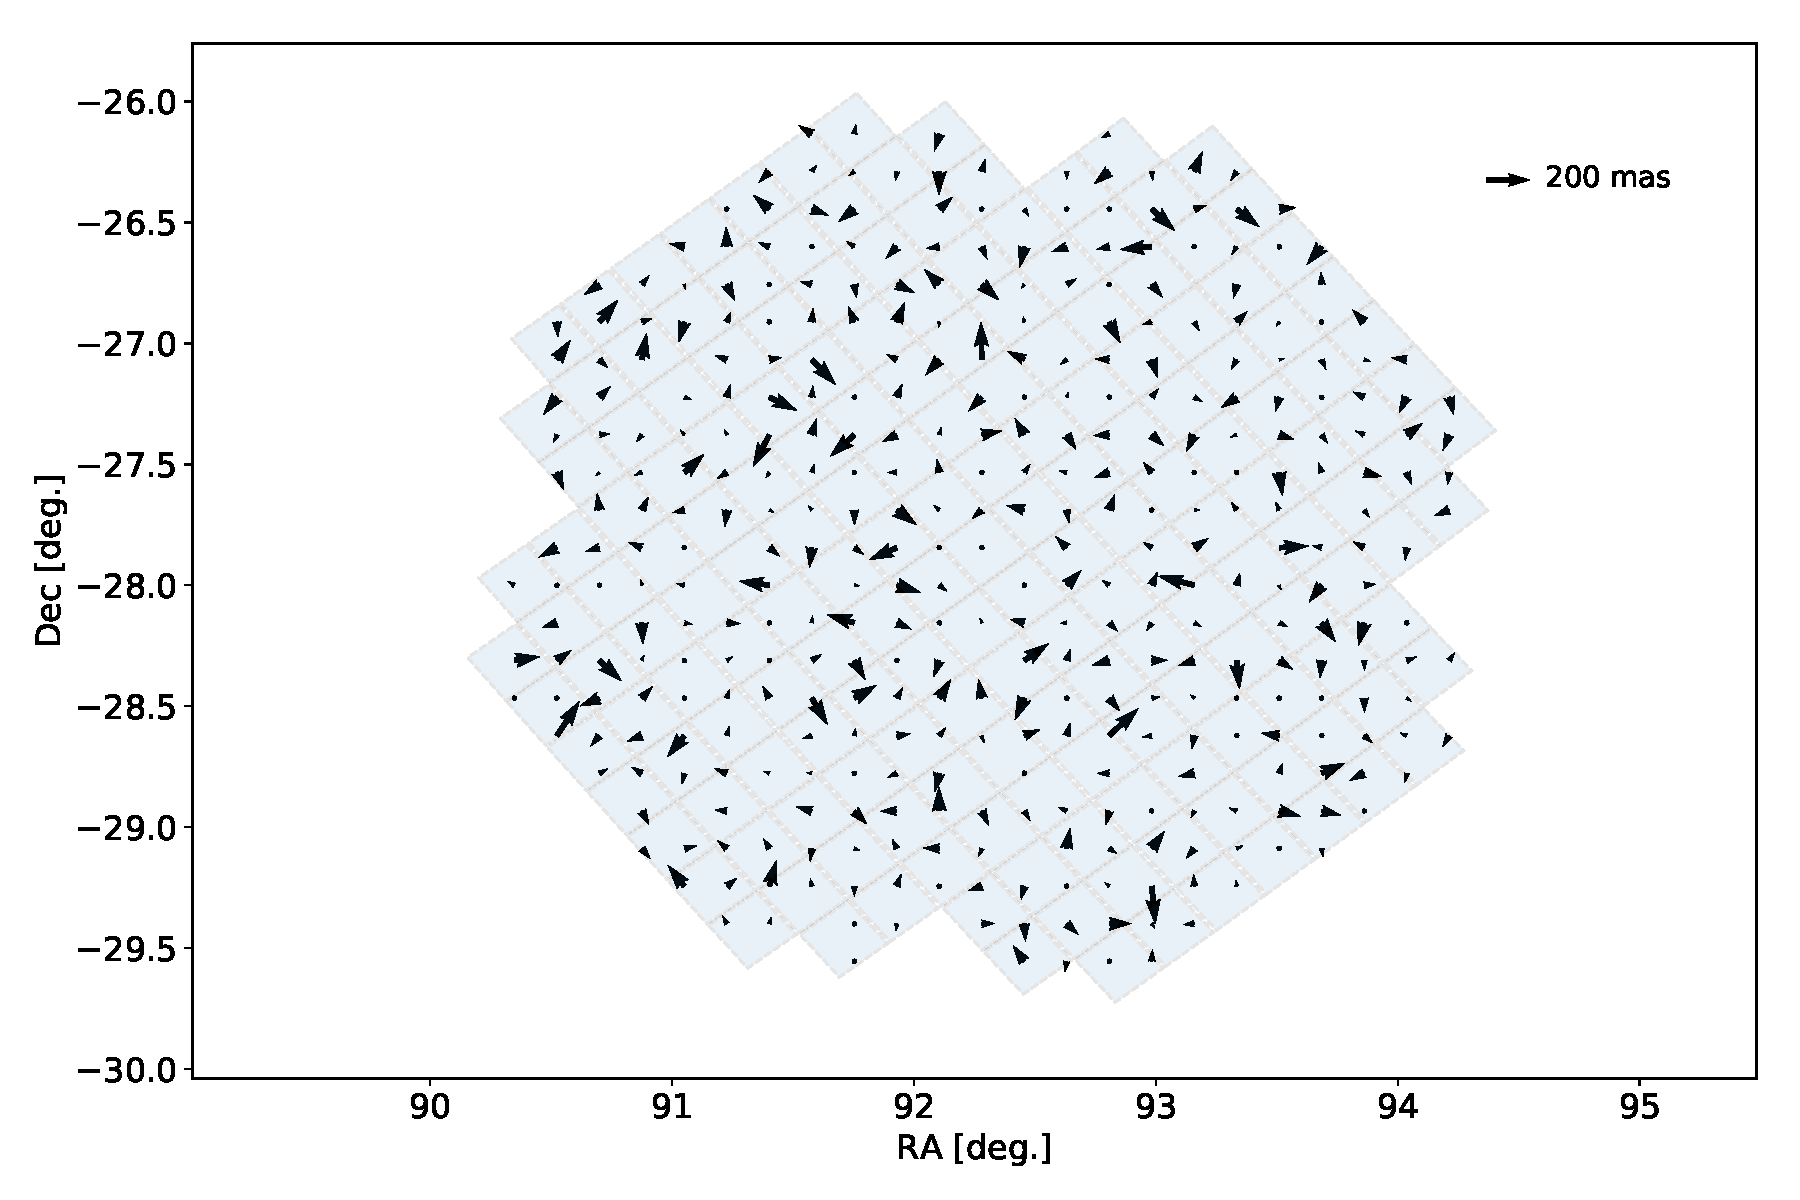
\includegraphics[width=0.45\textwidth]{astrometry_imsim_dithered_interp}
  \caption{Astrometic residuals measured in visit $270675$ from the imSim dithered run. The light blue squares represent the CCD chips in
  the LSST focal plane. The base of the arrow is on the input matched object. The arrows have been augmented by a factor 3600 for visualization purposes.}
  \label{fig:astrometry_c}
\end{figure}


\subsubsection{Internal checks}
\label{sec:internal_astrometry}

Another important test is to ensure the internal consistency of the astrometric solutions between different exposures. We select
a small region of the coadded area, which we will refer to as a \textit{patch}, and compare the positions of the objects detected in the coadd
image with the positions of objects detected in individual exposures that overlap with that patch.

In particular, we randomly choose 10 individual exposures and look for objects that fulfill the following criteria:
\begin{itemize}
  \item \texttt{deblend\_nChild==0}, the object has been completely deblended (it is a primary match).
  \item \texttt{base\_PixelFlags\_flag\_edge==0}, the object is not close to an edge.
  \item \texttt{base\_PixelFlags\_flag\_interpolatedCenter==0}, the object does not have any interpolated pixels in its center.
\end{itemize}

Note that, in this case, we are not requiring the objects to be classified as stars, we are omitting the cut in
\texttt{base\_ClassificationExtendedness\_value}, but we are adding some cuts to ensure that the objects were properly measured. Once
we perform our selection, the next step is to match the objects in the different exposures. To do so, we use the matching algorithm
included in the LSST software stack. We calculate the mean of the difference between the position of each source
in the coadd, $X_{coadd,i}$ and the position of the matched object in each of the exposures where it has been detected, $X_{visit_{j},i}$
for $j \in [1,10]$, i.e.,

\begin{equation}
  \Delta = \langle X_{coadd,i} - X_{visit_{j},i} \rangle
\end{equation}

We only consider matched objects detected in at least 5 exposures. The resulting distribution is shown in \figref{astrometry_internal}. We see that this distribution is noticeably narrower than those shown in \figref{astrometry_a} and \figref{astrometry_b} and no apparent bias is found, indicating that the processing is consistent among different epochs.

\begin{figure}
  \centering
  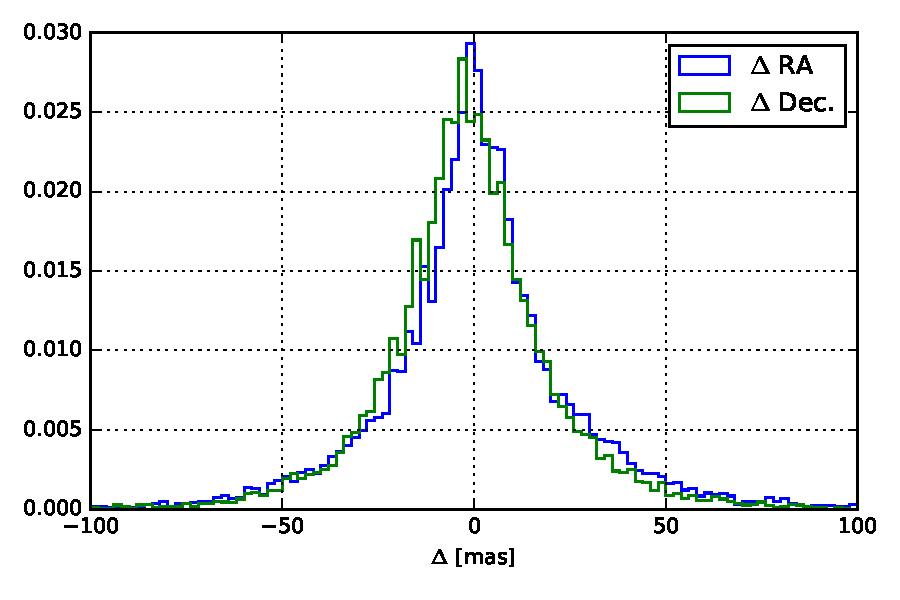
\includegraphics[width=0.45\textwidth]{astrometry_internal_10visits_imsim_undithered}
  \caption{Distribution of the mean difference in position (RA:blue, Dec:green) between the coadd and the different individual exposures
  where each source has been detected.}
  \label{fig:astrometry_internal}
\end{figure}

\subsection{Photometry checks}
\label{sec:photometry_checks}

As we did in previous sections, we perform two different tests to assess the quality of our simulations: first, we compare our output catalogs to the inputs, and second, we check the consistency between different visits for the same objects.

\subsubsection{External checks}
\label{sec:external_photometry}

We want to analyze the accuracy of the magnitude measurement by comparing the input catalog with the output catalog. This process not only checks
the accuracy of the measurement pipeline, but it also tests the quality and level of realism of the image generation pipeline.
For these external checks, we use the same 50 randomly selected visits from the previous section.
To study the photometric residuals, we use a different matching strategy compared to previous sections. In this case, we eliminate the threshold
in magnitude difference, looking for the input source that is closest in magnitude within a 0.2 arcseconds radius around each detected
source. In \figref{photometry_a} we can see the distribution of the photometric residuals. This distribution gets wider as we go
fainter (as expected). Furthermore, we see that the 0.02 magnitude selection cut is a good proxy to ensure that we account for most sources properly matched.

\begin{figure}
  \centering
  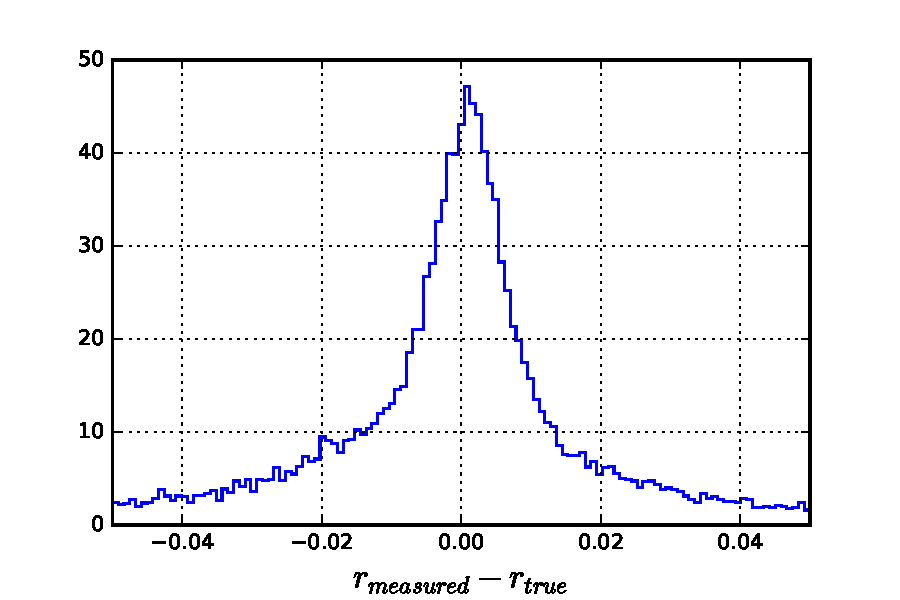
\includegraphics[width=0.45\textwidth]{photometry_imsim_dithered_50visits_hist}
  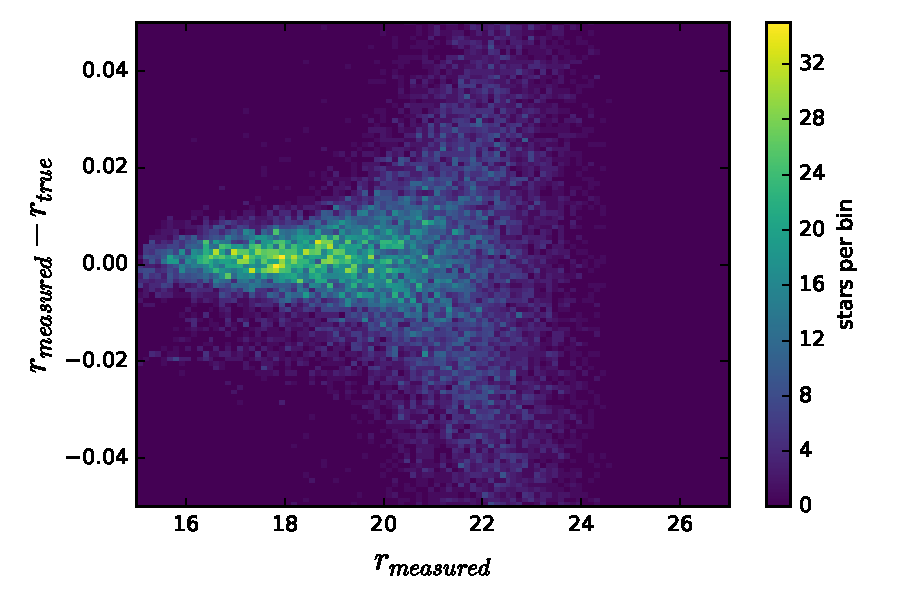
\includegraphics[width=0.45\textwidth]{photometry_imsim_dithered_50visits}
  \caption{Top: Distribution of magnitude difference between the input and output catalogs.
  Bottom: Difference magnitude between input and output catalogs as a function of the measured magnitude. We considered 50 visits
  randomly selected from the imSim dithered run. We find similar results for the imSim undithered run and for the PhoSim run.}
  \label{fig:photometry_a}
\end{figure}

\subsubsection{Internal checks}
\label{sec:internal_photometry}

We also checked the consistency of the photometry between different exposures. Using the same approach and sample presented in
\secref{internal_astrometry}, we compared the mean difference between the coadded source and 10 random single-visit images. In
principle, we would expect that some objects will show differences between different epochs due to their intrinsic variability, however,
these effects are not found in the inputs of the simulation for any of the objects, thus, the differences between different epochs are due to
statistical fluctuations and different observing conditions. The results from these checks are shown in \figref{internal_photometry_a}.

\begin{figure}
  \centering
  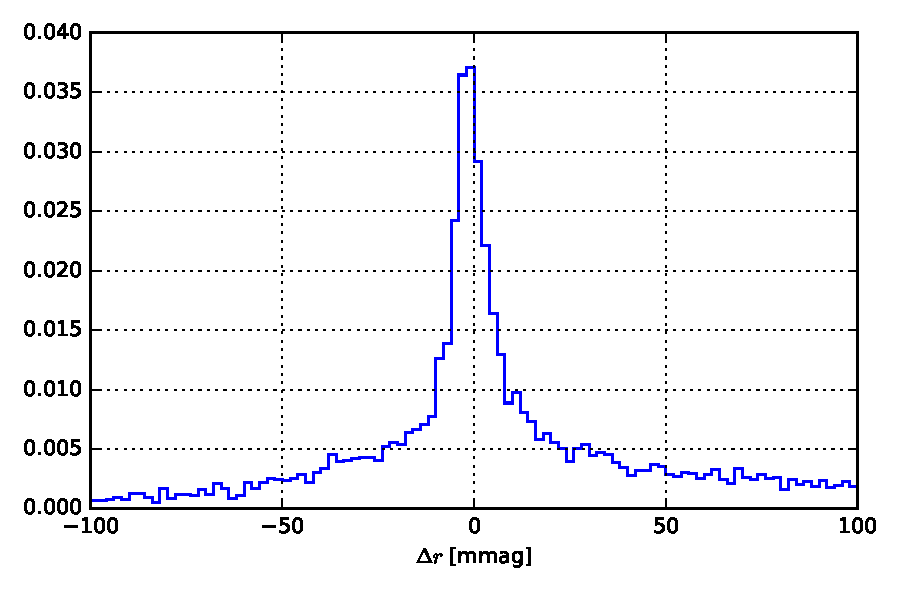
\includegraphics[width=0.45\textwidth]{photometry_internal_10visits_imsim_undithered}
  \caption{Distribution of the mean difference in magnitude between the coadd and the different individual exposures
  where each source has been detected. The mean of the distribution is consistent with zero.}
  \label{fig:internal_photometry_a}
\end{figure}

In this figure, we see that the mean of the distribution is compatible with zero and that most sources have a magnitude difference lower
than 25 mmag given the narrow peak. The presence of long tails are likely due to blends and mismatching or artifacts.

\subsection{PSF checks}
\label{sec:psf_checks}

In order to ensure the accuracy of shape measurements a robust and accurate estimation of the PSF is required. In the case of imSim, we have
an analytical input PSF that only depends on the airmass at the time of observation. We can check if the measurement pipeline can reconstruct
the input PSF. To do so, we select 200 visits randomly, retrieve the measured PSF using the pipeline, and compare this
to the input model given the observing conditions. We obtain the residual depicted in \figref{psf_residual}, where we see that the PSF model residuals are very small in the center of the image and that the tails are dominated by noise.

\begin{figure}
\centering
\begin{tikzpicture}
  \node[inner sep=0pt] (A) {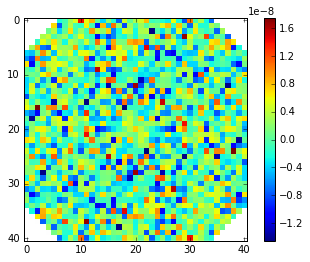
\includegraphics[width=0.9\columnwidth]{psf_residual.png}};
  \node[black] (B) at ($(A.south)!-.01!(A.north)$) {X [pixels]};
  \node[black,rotate=90] (C) at ($(A.west)!-.01!(A.east)$) {Y [pixels]};
  \node[black,rotate=90] at ({$(A.west)!1.0!(A.east)$} |- {$(A.south)!.55!(A.north)$}) {PSF$_{output}-$PSF$_{input}$};
\end{tikzpicture}

\caption{Average difference between the input PSF model (41$\times$41 pixels, normalized to unity) and the measured PSF (with the same normalization) for 200 visits.}
\label{fig:psf_residual}
\end{figure}

\subsection{LSST Science Requirements Document Key Performance Metrics}

We processed the output individual-visit catalogs through the LSST Project package \texttt{validate\_drp}\footnote{\url{dmtn-0008.lsst.io}}\footnote{\url{https://github.com/lsst/validate_drp}}
The \texttt{validate\_drp} package calculates the Key Performance Metrics (KPMs) from the LSST Science Requirements Document (SRD)~\citep{LPM-17}.

Given the simplified and somewhat idealized nature of the DC1 simulations, we expect that the DC1 should pass the SRD KPMs.

The photometric repeatability (PA1) is 6~mmag as measured by the inter-quartile range.  The ultimate design goal is 5~mmag.  The 6~mmag is dominated by a tail of scattered objects, see \figref{validate_drp_check_photometry}.

The photometric error model from \citet[][Eq. 6,7]{Overview} is
\begin{eqnarray}
\sigma^2 = \sigma^2_{\rm sys} \sigma^2_{\rm rand} \\
\sigma^2_{\rm rand} = (0.04 - \gamma) 10^{0.4(m-m_5)} + \gamma 10^{0.8(m-m_5)}
\label{eq:photometric_error}
\end{eqnarray}
where $\gamma$ describes noise from the sky and detector electronics, and the 5-$\sigma$ point-source depth is given by:
\begin{equation}
\begin{split}
m_5 = C_m + 0.50 (m_{\rm sky} - 21~{\rm mag/{\rm arcsec}^2}) \\
+ 2.5 \log_{10} (0.7{\arcsec}/\theta_{\rm eff}) \\
+ 1.25 \log_{10} (t_{\rm vis} / 30~{\rm s}) - k_m (X-1)
\label{eq:photometric_m5}
\end{split}
\end{equation}
where $C_m$ summarizes the throughput of the telescope optics and camera, $m_{\rm sky}$ is the sky brightness, $\theta_{\rm eff}$ is the seeing, $t_{\rm vis}$ is the exposure time, $k_m$ is the airmass coefficient, and $X$ is the airmass.

Our fits find $m_5$ = 24.2~mag/arcsec$^2$ and $\gamma=0.038$ which are quite consistent with the \citet[][Table 2]{Overview} values of $m_5=24.35$~mag/arcsec$^2$, $\gamma=0.039$.  This demonstrates that generate simulations of the telescope, detector, and sky in accordance with the \citet{Overview} estimates.

Note that we find $\sigma_{\rm sys}=0$~mmag, which is consistent with the idealized simulations we run for DC1 with no additional systematic sources of errors.

\begin{figure}
\centering
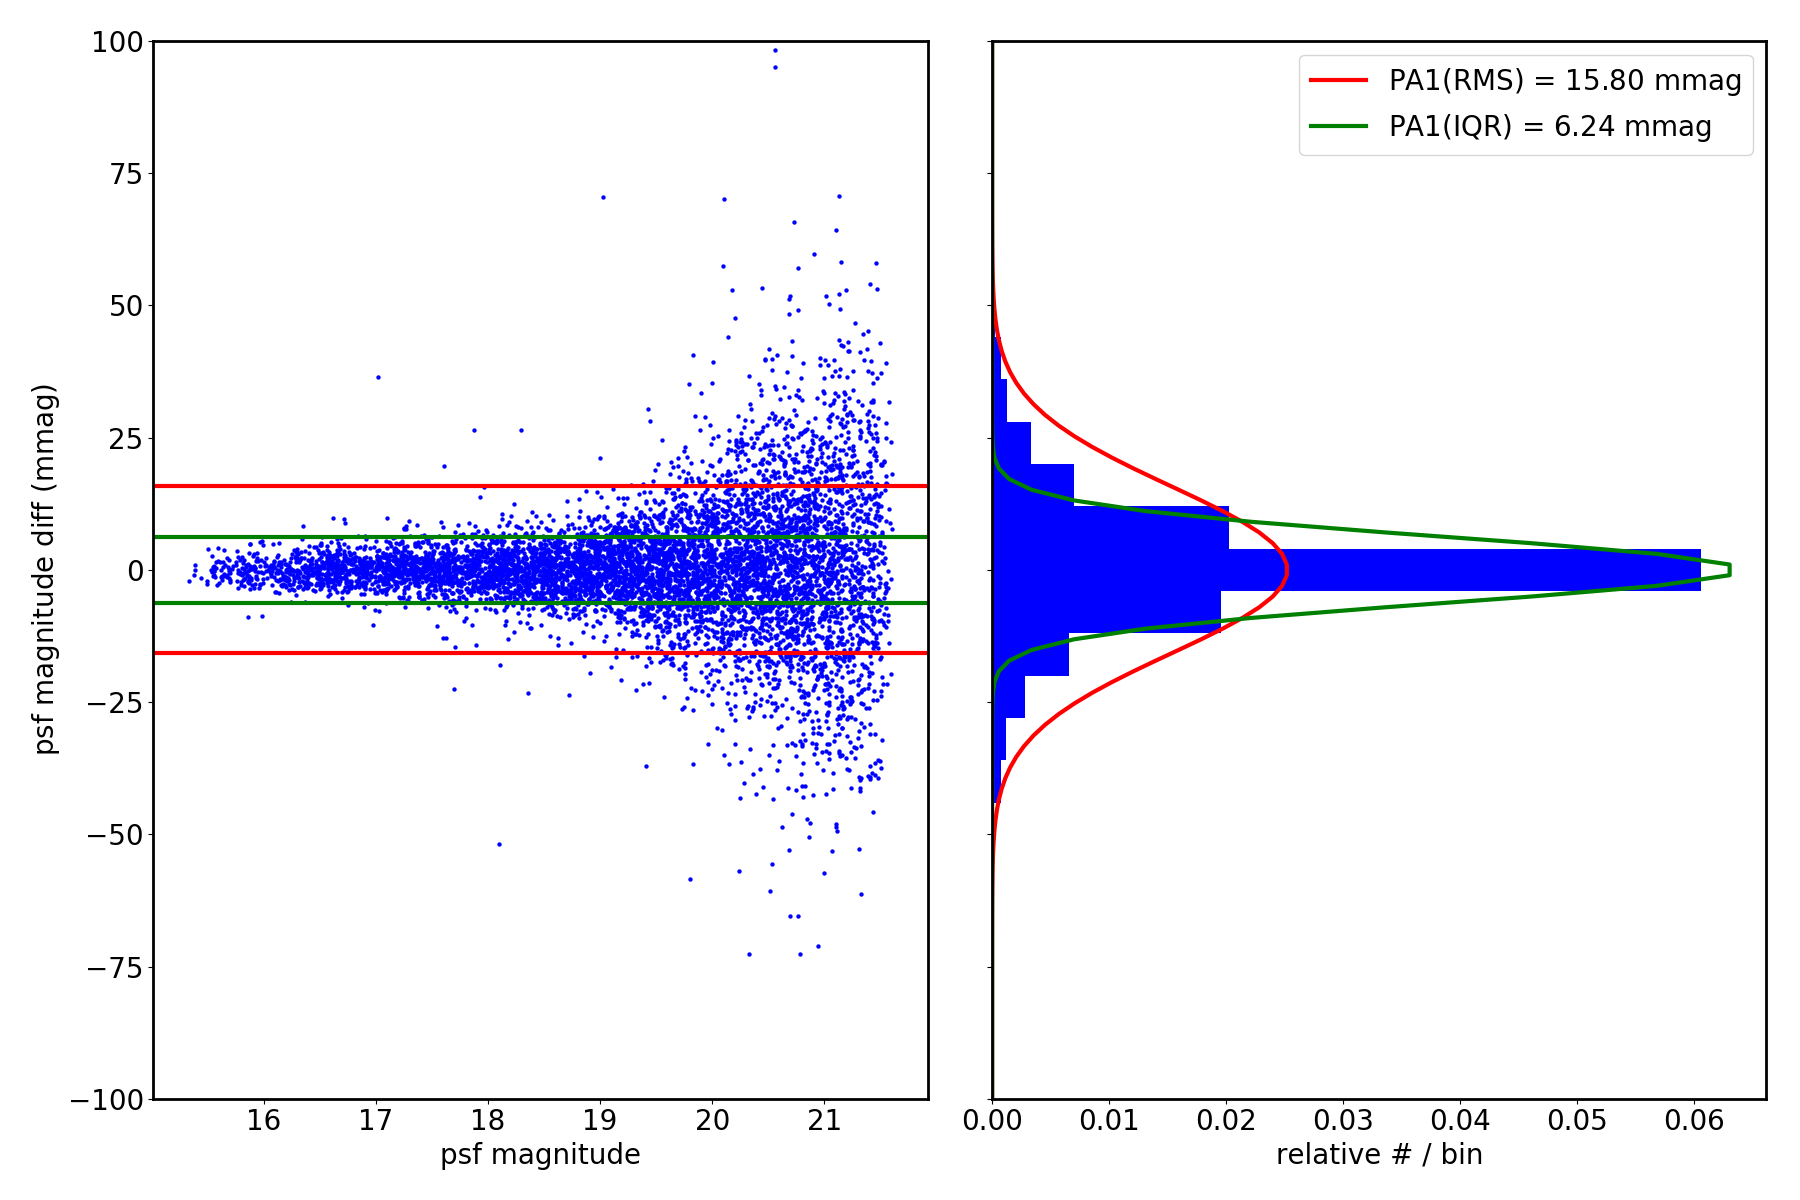
\includegraphics[width=0.9\columnwidth]{DC1-imsim-dithered_r_PA1.png}
\caption{(left) The magnitude difference of pairs of measurements of stars across visits for stars with a typical signal-to-noise ratio $>100$.  (right) The histogram of these differences.  The gaussian RMS is shown in red while the inter-quartile range (rescaled to match a gaussian RMS) is shown in green.  Note that the distribution is more peaked than a gaussian.  The IQR (6.2~mmag) is {\em smaller} than the gaussian RMS (15.8~mmag).}
\label{fig:validate_drp_PA1}
\end{figure}

\begin{figure}
\centering
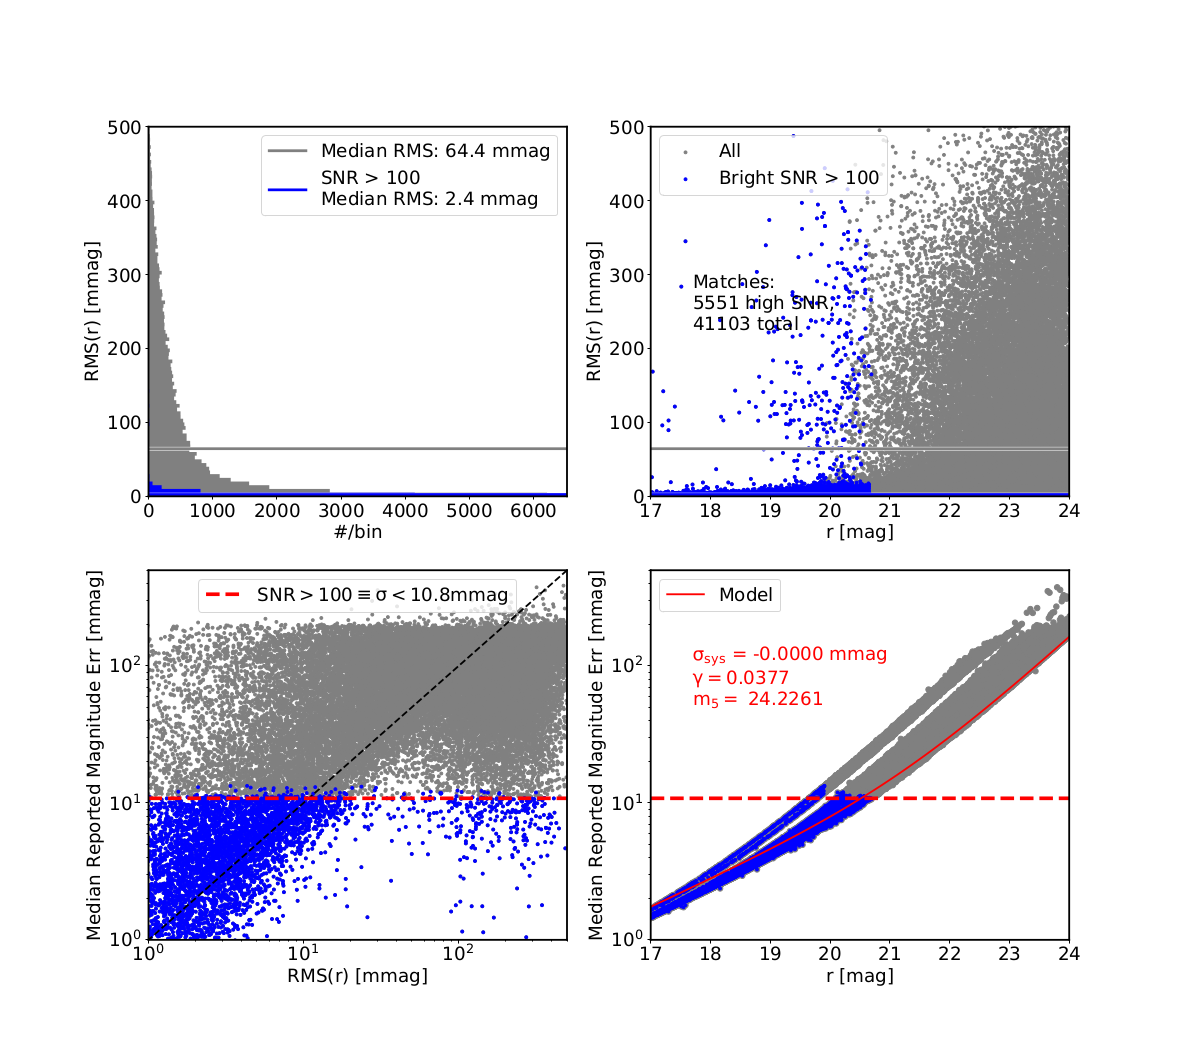
\includegraphics[width=0.9\columnwidth]{DC1-imsim-dithered_r_check_photometry.png}
\caption{Photometric performance in more detail.  (upper left) Horizontal histogram of the RMS distribution for each star for the full sample (grey) and ``bright'' sample (blue).  The blue sample is the same as that shown in Figure.~\ref{fig:validate_drp_PA1}.
(upper right).  Note that this RMS is the RMS of the measurements for a given star and so each entry in the histogram is one star.  Thus the median value here is 2.4~mmag, even thought the median of all RMS measurements in Figure.~\ref{fig:validate_drp_PA1} was 15.8~mmag.  This difference is due to a population of objects that have a poor repeatability.
(upper right) The RMS distribution as a function of magnitude of the star.  Here you can see the tight core of very repeatable measurements, along with a smaller population of objects with much higher scatter to their measurements.
(lower left) Per-object median reported magnitude error by the pipeline versus the observed RMS over all of the measurements for an object.  Our $SNR>100$ cut is in the space of median reported error.
(lower right)
Per-object median pipeline-reported magnitude error versus object magnitude.
 {\bf TODO: MWV CLEANUP (1) title, (2) incorrect xlabel (should be \#/bin),  and "Filter name" extra text}
 {\bf TODO: MWV  Are these higher scatter objects galaxies, stars in halos of bright stars, additionally added objects that were done inconsistently with the rest of the catalog?}
 {\bf TODO: MWV  The lower-left plot has never actually made sense to me.  I should investigate this
   more.} \rachel{I recommend making this a page-width rather than column-width figure.}}

\label{fig:validate_drp_check_photometry}
\end{figure}


\begin{figure}
\centering
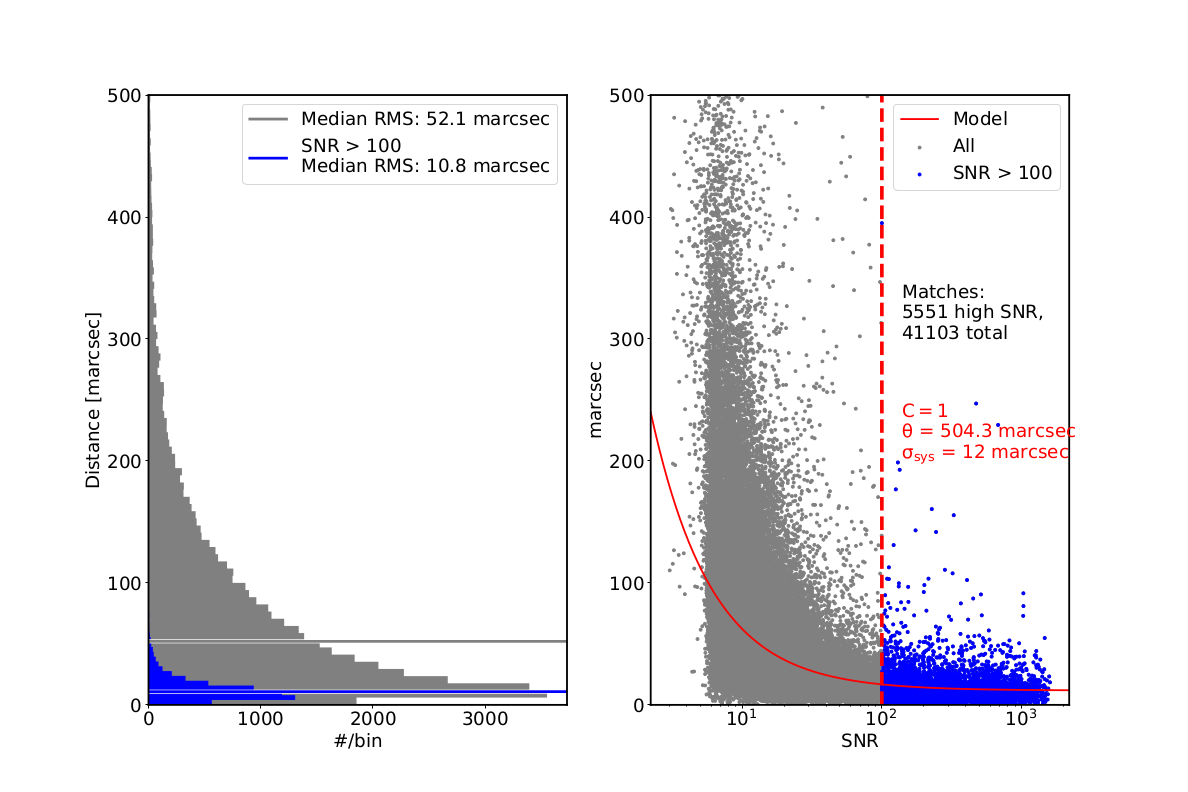
\includegraphics[width=0.9\columnwidth]{DC1-imsim-dithered_r_check_astrometry.png}
\caption{
Detailed astrometric performance.  (left) Histogram of the repeatability of distance between pairs of stars.  (right) Astrometric variation as a function of SNR.  We find a systematic floor of 12~milliarcsec.
{\bf TODO: MWV CLEANUP (1) title, (2) fix xlabel, which should be \#/bin}
{\bf TODO: MWV IS THIS HISTOGRAM DIFFERENT THAN THE check\_photometry histogram in terms of per-pair vs. per-object variation.}}
\label{fig:validate_drp_check_astrometry}
\end{figure}

\begin{figure}
\centering
\includegraphics[width=0.9\columnwidth]{{DC1-imsim-dithered_r_validate_drp.AM1_D_5_arcmin_17.0_21.5_mag}.png}
\includegraphics[width=0.9\columnwidth]{{DC1-imsim-dithered_r_validate_drp.AM2_D_20_arcmin_17.0_21.5_mag}.png}
\includegraphics[width=0.9\columnwidth]{{DC1-imsim-dithered_r_validate_drp.AM3_D_200_arcmin_17.0_21.5_mag}.png}
\caption{
Astrometric repeatibility: variation in distances measurement between pairs of stars at (top) 4-6$\arcmin$, (middle) 19-21$\arcmin$, (bottom) 199-201$\arcmin$.  AM(1,2,3) are the distance measurements, while AF(1,2,3) are the fraction of pairs lying outside the a specified limit.
The performance is excellent, with characteristic values all below the LSST SRD levels.
{\bf TODO: MWV CLEANUP}
 {\bf TODO: MWV ADD ADx values to interpret AFx values}}
\label{fig:validate_drp_AMx}
\end{figure}

{\bf TODO: MWV Add table of performance metrics}

\section{Analysis of the simulated dataset}
\label{sec:analysis}
In this section, we analyze the clustering properties of our output catalog from the end-to-end pipeline and compare with the input catalog.

\subsection{Matching input and output catalogs}
\label{sec:matching}

End-to-end simulations, can potentially allow us to trace each measured photon to its corresponding source in order to characterize the measurement process, however this requires large overhead storage. 

%A simple way to trace the photons could be storing each postage stamp for the different sources in different exposures. The problem with this approach is that it also requires a large additional storage space. Generating efficient strategies to perform this bookkeeping and connecting input and output catalogs is an important research topic for end-to-end simulations, however it is out of the scope of this work.

The simplest way to connect two catalogs is by using the positions of the objects in the sky. This approach has been extensively used in the literature~\citep{1977A&AS...28..211D,1983Obs...103..150B,1986MNRAS.223..279W} and performs reasonably well when blending is low, since the probability of confusing two objects is small. However, when blending is high, this approach might be not be sufficient. Then, matching other quantities like flux or shape can become useful~\citep{2008ApJ...679..301B}.

We compare two different matching strategies: positional matching, where we match the find the objects in the truth catalog closest to the detected objects, which we will refer to as \textit{pure spatial matching}; and positional matching including magnitude matching, which we will refer to as \textit{spatial+magnitude matching}, where for each detected object we find objects from the input catalog that lie within one pixel radius ($0.2 \arcsec$). After this, we select the object that is closest in magnitude as long as the difference in magnitude is less than a certain threshold. In our case, we arbitrarily chose $0.5$. If any of these conditions are not fulfilled, then the object is considered not matched.

In the first approach, all detected objects are matched to an object in the input catalog where, in principle, the two point statistics should be preserved between the catalogs. In the second approach, we can potentially bias the results since we omit sources where the accuracy in the magnitude measurement is low. To compare both approaches, we check the possible biases in the measured magnitude $\Delta$mag = mag$_{meas} - $mag$_{true}$. In \figref{matching_comparison}, we see that spatial matching is enough to get a good match in magnitude as evidenced by the median value of $\Delta$mag compared with the spatial+magnitude matching. This figure also shows that spatial matching is more affected by the presence of outliers than the spatial+magnitude matching, as expected by the clipping performed on the latter. The evolution of the mean and median $\Delta$mag with the magnitude shows that brighter objects with magnitudes $\sim 18-21$ appear usually brighter and, on the other hand, fainter objects with magnitudes $\sim 23-25$ appear dimmer. This is likely a consequence of the deblender assigning a larger flux to the brightest members of the blend, while the fainter members seem to lose flux. Finally, since for the faintest end (mag $\sim 26$) we can only detect those that appear brighter (thanks to the background noise) than they actually are. This results in a negative value for the mean and median $\Delta$mag.

\begin{figure}
\centering
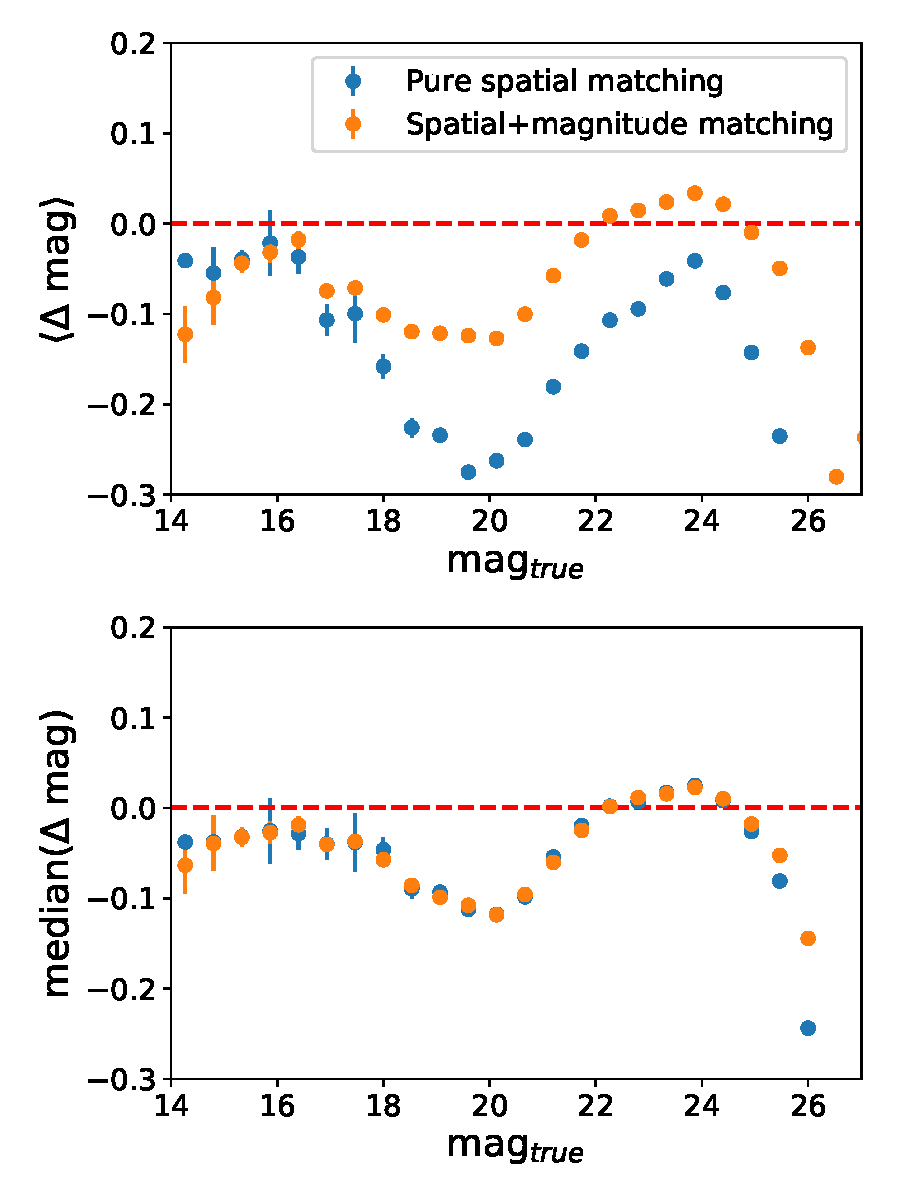
\includegraphics[width=0.9\columnwidth]{matching_comparison_galaxies.pdf}
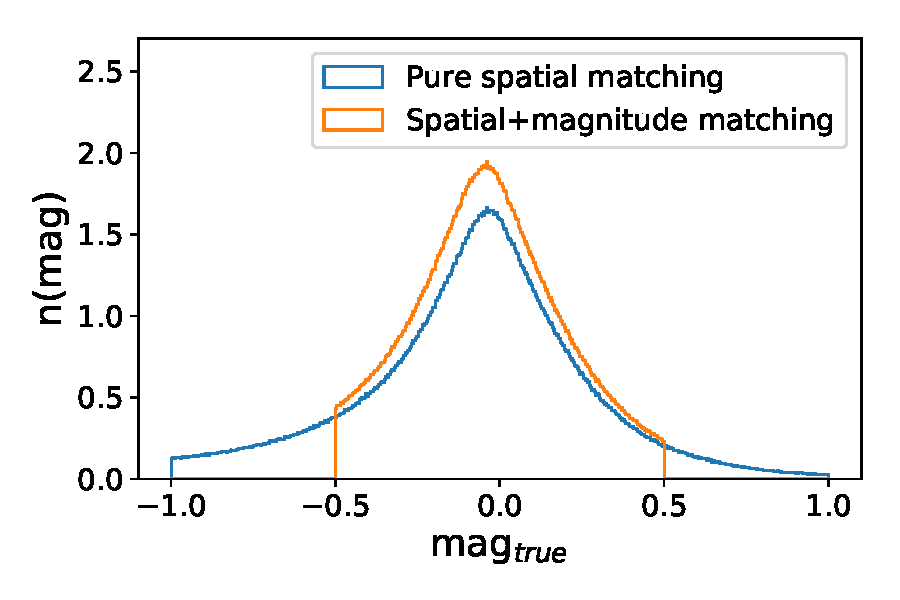
\includegraphics[width=0.9\columnwidth]{mag_hist_total.pdf}
\caption{Mean (top), and median (middle) of $\Delta$mag as a function of the true magnitude, with pure spatial matching (blue) and spatial+magnitude matching (orange). Bottom: Histogram of $\Delta$ mag.}
\label{fig:matching_comparison}
\end{figure}

We also compared the power-spectra of the detected objects and the matched input objects in \figref{matching_cls}. We see that the spatial matching recovers the power-spectrum well, with some wiggling at very low scales due to mismatches and small differences in position between the detected and the input catalogs. In the case of spatial+magnitude matching, we see that the power for the matched catalog is consistently lower. This is due to objects that are detected but not matched to any object in the true catalog, since this effect disappears when we just consider the objects that have been matched.

\begin{figure}
\centering
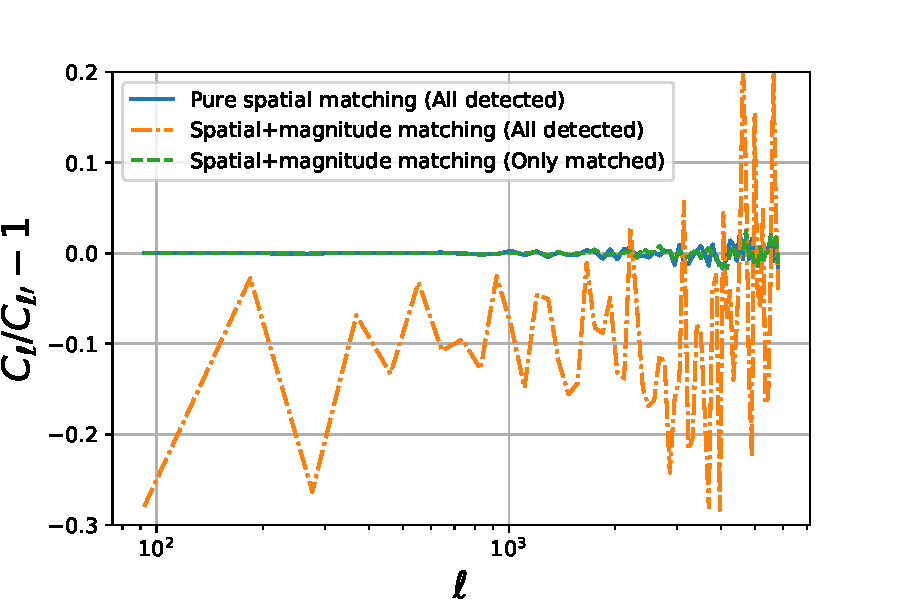
\includegraphics[width=0.9\columnwidth]{cl_comparison_matching.pdf}
\caption{Relative difference between the power-spectrum measured for the detected objects and the matched objects in the input catalog with spatial matching compared to all detected objects (blue, solid line), spatial+magnitude matching compared to all detected objects (orange, dash dotted line), and spatial+magnitude matching compared to matched objects using this schema (green dashed line).}
\label{fig:matching_cls}
\end{figure}

The problem with these matching techniques is the lack of details about blended objects. For analyses involving blending and/or very small scale information, different approaches should be considered.

% ----------------------------------------------------------------------

\subsection{Generating depth maps}
\label{sec:masking}

In order to estimate the depth in the coadd catalogs, we select stars using the extendedness-based classifier: \texttt{base\_ClassificationExtendedness\_value==0}. This ensures selecting
PSF-like objects. After this, we use two different approaches:

\begin{enumerate}
\item In the first approach we generate a HEALPix\footnote{\url{http://healpix.sf.net}}~\citep{2005ApJ...622..759G} map containing the PSF-like objects detected with a signal-to-noise ratio (SNR) $\geq 5$ (\texttt{base\_PsfFlux\_flux/base\_PsfFlux\_fluxSigma>=5}), and we assign to each HEALPix pixel the value of the
dimmest object contained in it. We will refer to this method as method \#1.
\item The second procedure also generates a HEALPix map containing the PSF-like objects. Here, for each HEALPix pixel, we compute the median SNR as a function of the magnitude and use the magnitude at which SNR is closest to 5. We will refere to this method as method \#2.
\end{enumerate}

These two procedures yield very similar results (within $\sim 4\%$). We show the relative difference in \figref{depth_maps}. We also check that the maps built selecting galaxies instead of stars are compatible as well. We will select our footprint according to the depth map using the second methodology. These maps are also shown in \figref{depth_maps}.

\begin{figure*}
\centering
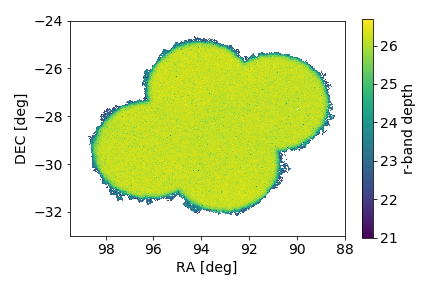
\includegraphics[width=0.45\textwidth]{dithered_depth.png}
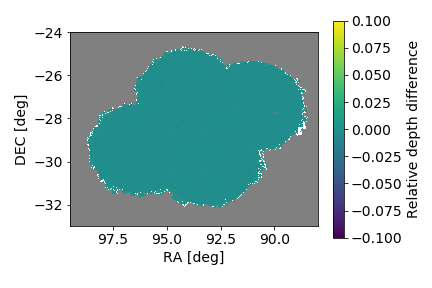
\includegraphics[width=0.45\textwidth]{dithered_difference.png}
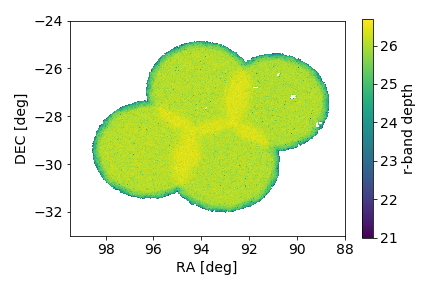
\includegraphics[width=0.45\textwidth]{undithered_depth.png}
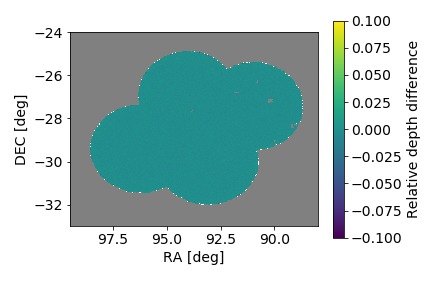
\includegraphics[width=0.45\textwidth]{undithered_difference.png}
\caption{Left column: 5-$\sigma$ depth for the dithered (top) and undithered (bottom) fields using the method \#2 in the text. Right column: Relative difference between the depth estimated using the methods presented in the text for the dithered (top) and undithered (bottom) fields.}
\label{fig:depth_maps}
\end{figure*}

\subsection{Bright objects masking and data selection}

Bright objects produce significant effects in the image that affect the detection and measurement of neighboring objects. Some examples of these effects include saturation, large diffraction spikes, obscuration of neighboring sources, etc. Thus, masking a region around these sources creates a more complicated footprint but greatly simplifies the analysis of systematic effects. In order to evaluate the effects from these sources, we take the stars from the input catalog, bin them according to their magnitude, and count the number of sources detected in a given radius. One caveat is that the number of stars in an aperture of radius $\theta_{1} > \theta_{0}$, depends on the number of stars on the aperture with radius $\theta_{0}$. Therefore, it is better to use a differential measurement. Results of this are shown in \figref{galdens_derivative}. We see that there is an excess of sources at distances lower than 10 arcseconds for the brightest stars. This is mainly due to the shredding of these bright sources around their outskirts. Bright noisy pixels are detected as individual (point-like) sources resulting in fake source detections. On the other hand, we do not see any obscuration present on scales that we are interested in (1 arcmin and higher). We conclude that no additional masking is required but a careful object selection becomes important for clustering analyses.

\begin{figure}
\centering
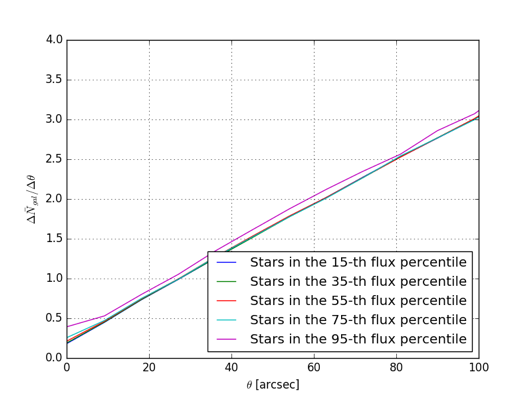
\includegraphics[width=0.9\columnwidth]{dngal_dtheta.png}
\caption{Mean increment in the number of detected objects around stars in the 95th flux percentile (magenta), the 75th percentile (cyan), the 55th percentile (red), the 35th percentile (green) and the 15th percentile (blue). We see that for the brightest percentiles there is no obscuration present but a overdensity of targets. These are mainly noise peaks identified as point sources.}
\label{fig:galdens_derivative}
\end{figure}

We also check the detection efficiency of galaxies in our sample. We selected galaxies in the catalog using the variable \texttt{base\_ClassificationExtendedness\_value} as a star/galaxy separator (as in \citet{2017arXiv170506766B}). Objects where this variable is equal to 1 are more likely to be galaxies, whereas the objects where it is 0 are more likely to be stars. We also make some quality cuts by selecting the objects with \texttt{detect\_isPrimary==True}. The selection in this variable ensures that the object has been fully deblended and that the detection was not close to the edge of a coadded image. The results are in \figref{completeness}, where we compute the ratio of detected objects classified as galaxies and the input number of galaxies, $\varepsilon$, as a function of magnitude. We check this ratio for both the dithered and undithered catalogs and in pixels where the depths were higher than 25.7 and 26.25. We used \texttt{CMODEL\_MAG} as the reference magnitude for the detected objects and the true magnitude for the input galaxies.

\begin{figure}
\centering
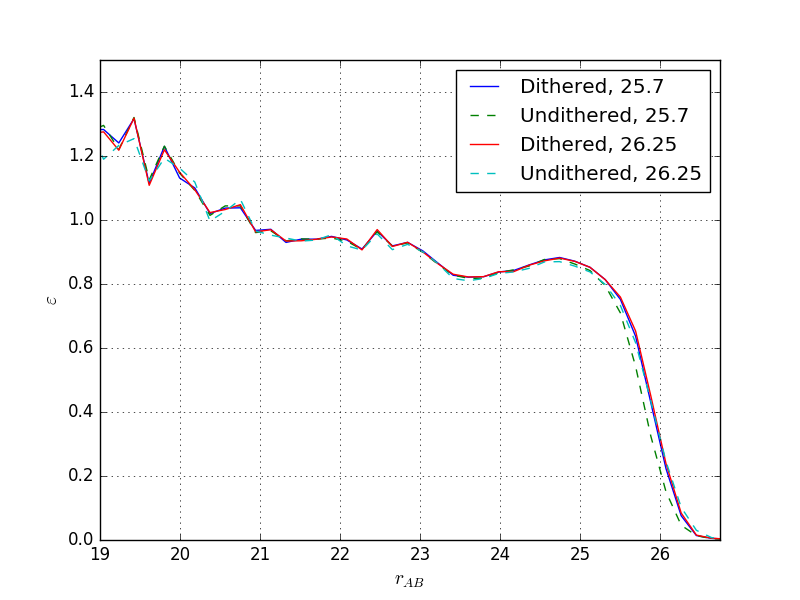
\includegraphics[width=0.9\columnwidth]{completeness.png}
\caption{Number of detected objects classified as galaxies divided by the number input galaxies as a function of magnitude. We see that the detection efficiency is larger than 80\% for the most part and a considerable fraction of objects with magnitude lower than 20 are being misclassified.}
\label{fig:completeness}
\end{figure}

\figref{completeness} shows that selecting galaxies with \texttt{base\_ClassificationExtendedness\_value==1}, \texttt{detect\_isPrimary==True} and \texttt{CMODEL\_MAG $>$ 21} is enough to get rid of most potential problems with fake source detections. We confirmed this by performing visual inspection on the images. We noticed that fake sources happen close to very bright objects. In addition, it seems that selecting \texttt{CMODEL\_MAG $<$ 25.3} ensures high completeness ($\sim 80\%$). Uniformity is ensured by selecting the galaxies that lie within HEALPixels where the depth is $\geq 25.3$. After these selection cuts, we obtain 4.4 million galaxies for the dithered field and 4.3 for the undithered field.
% ----------------------------------------------------------------------

\subsection{Clustering results}
\label{sec:results}

In this section, we analyze the two point clustering statistics for both the dithered and undithered catalogs in real and harmonic space and check the consistency between the input and measured observables. When comparing the input and output catalogs, some subtleties arise. For example, selecting a galaxy sample in the input catalog with $m_{low} < m_{true} < m_{high}$, where $m_{low}$ is the lower $r$-band magnitude threshold, $m_{true}$ is the true $r$-band magnitude of the object and $m_{high}$ is the upper $r$-band magnitude threshold, and a second galaxy sample in the output catalog with $m_{low} < m_{measured} < m_{high}$, with $m_{measured}$ being the $r$-band measured magnitude, results in a different power-spectra. The power spectrum in the first (selected according to true magnitude) sample will have a larger overall power than the second (selected according to measured magnitude) sample. This is due to the fact that the second sample includes galaxies that reach fainter, resulting in a wider window function. 

\subsection{2-point correlation function}
Using the samples presented in previous sections, we measure the 2-point correlation function using \texttt{TreeCorr}~\citep{2004MNRAS.352..338J}, selecting the Landy \& Szalay estimator~\citep{1993ApJ...412...64L},

\begin{equation}
w(\theta) = \frac{DD - 2 DR + RR}{RR}
\end{equation}
where $DD, DR$, and $RR$ are the number of pairs of objects from the data $D$ or the random catalog $R$ that cover the footprint. We use 30 angular log-spaced bins between $\theta=0.0001^{\circ}$ and $\theta=10^{\circ}$. We choose the number of bins so that the resulting covariance matrix is nearly diagonal. The covariance matrices are calculated using the delete-one jackknife technique~\citep{Shao:1986:DJB,2009MNRAS.396...19N}. We divide the footprint in $N_{JK}=100$ regions. These regions are defined using the K-means algorithm from the package \texttt{kmeans\_radec}\footnote{\url{https://github.com/esheldon/kmeans\_radec}}. The covariance matrix is computed as
\begin{equation}
\mathrm{Cov}_{JK}(\theta_{i},\theta_{j})=\frac{N_{JK}-1}{N_{JK}}\sum_{k=1}^{N_{JK}}\Delta w_{k}(\theta_{i}) \Delta w_{k}(\theta_{j})
\end{equation}
\begin{equation}
\Delta w_{k}(\theta_{i}) = w_{k}(\theta_{i})-\bar{w}(\theta_{i})
\end{equation}
where $w_{k}(\theta_{i})$ is the value of the correlation function when deleting the $k$-th region at the scale $\theta_{i}$, and $\bar{w}(\theta_{i})$ is the average correlation function at that same scale. We compute the correlation function on the dithered and undithered catalogs using their respective footprints, and we compare with the predicted correlation function given the $N(z)$ obtained by the spatial matching presented in previous sections, using \texttt{CCL}\footnote{https://github.com/LSSTDESC/CCL}~\citep{CCL}. The results are shown at \figref{2pt_corr}. We find that both measurements are in good agreement and in agreement with the theoretical prediction for $\theta < 0.3$ degrees. The angular range is mainly limited by our surveyed area.

\begin{figure}
\centering
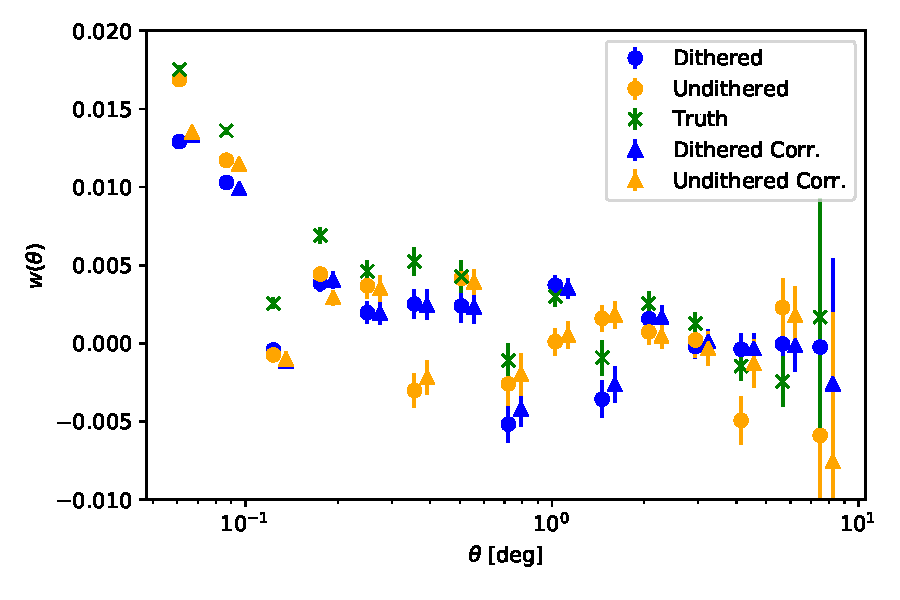
\includegraphics[width=0.9\columnwidth]{w_comp_corr25p3.pdf}
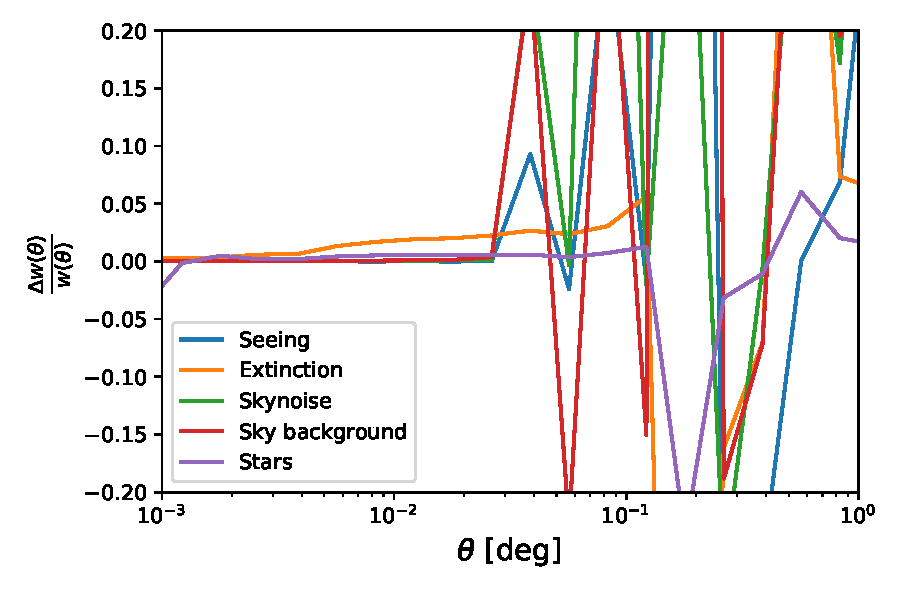
\includegraphics[width=0.9\columnwidth]{sys_dithered_25p3_v2.pdf}
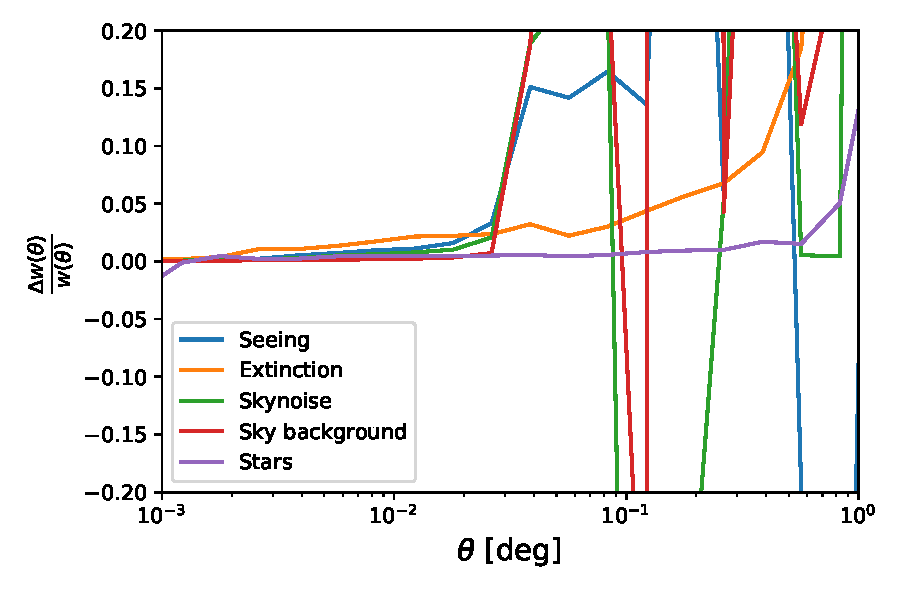
\includegraphics[width=0.9\columnwidth]{sys_undithered_25p3_v2.pdf}
\caption{{\bf Top panel:} Results for the two-point correlation function in the input (green), dithered (blue) and undithered (orange) datasets. We can see that after the correction (triangles) for the systematic effects, presented in Section \ref{ssec:systematics}, the agreement is better than without the correction (circles) between the input and output data especially for the undithered case (for the dithered case the corrections are negligible). {\bf Middle and bottom panels:} Correction due to the different potential sources of systematic uncertainty relative to the value of the measured correlation function of the dithered (middle panel) and undithered (bottom panel) datasets. We show that the correction is at percent level for $\theta<0.03$ degrees and grows beyond the $20\%$ level for $\theta \approx 0.1$ degrees.}
\label{fig:2pt_corr}
\end{figure}

%\begin{figure}
%\centering
%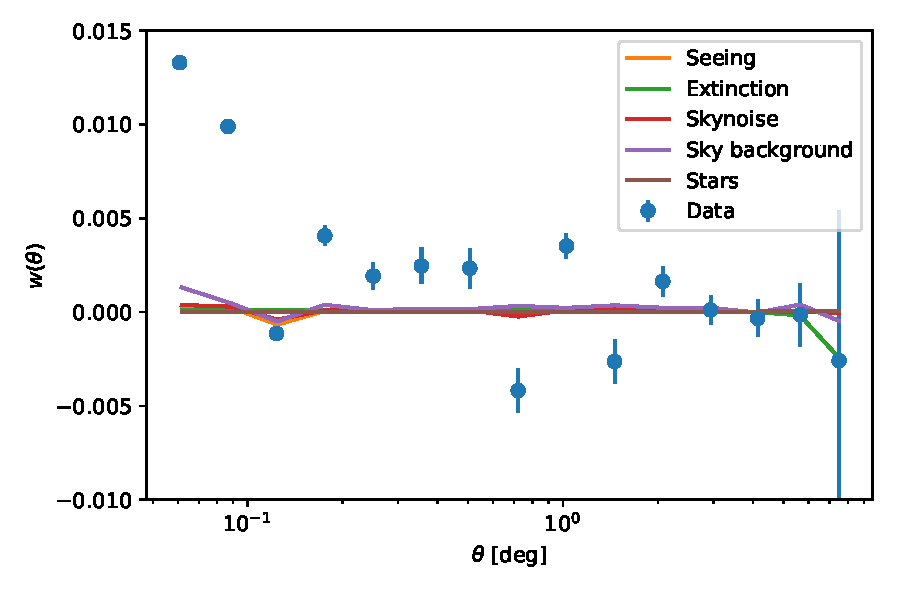
\includegraphics[width=0.9\columnwidth]{w_dithered_25p3.pdf}
%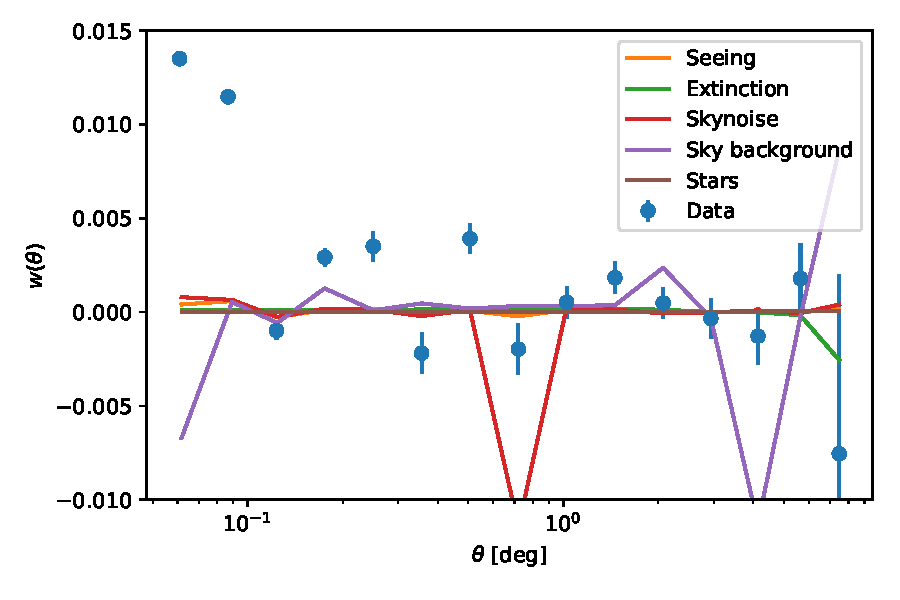
\includegraphics[width=0.9\columnwidth]{w_undithered_25p3.pdf}

%\caption{Correction due to the different potential sources of systematic uncertainty relative to the value of the measured correlation function of the dithered (top) and undithered (bottom) datasets. We show that the correction is at percent level for $\theta<0.03$ degrees and grows beyond the $20\%$ level for $\theta \approx 0.1$ degrees.}
%\label{fig:sys_realspace}
%\end{figure}


%We also show the correlation matrix,
%\begin{equation}
%\mathrm{Corr}_{ij}=\frac{\mathrm{Cov}_{ij}}{\sqrt{\mathrm{Cov}_{ii}\mathrm{Cov}_{jj}}}
%\end{equation}
%in \figref{2pt_cov} where we can see that in both cases the matrices are almost diagonal.
%\begin{figure}
%\centering
%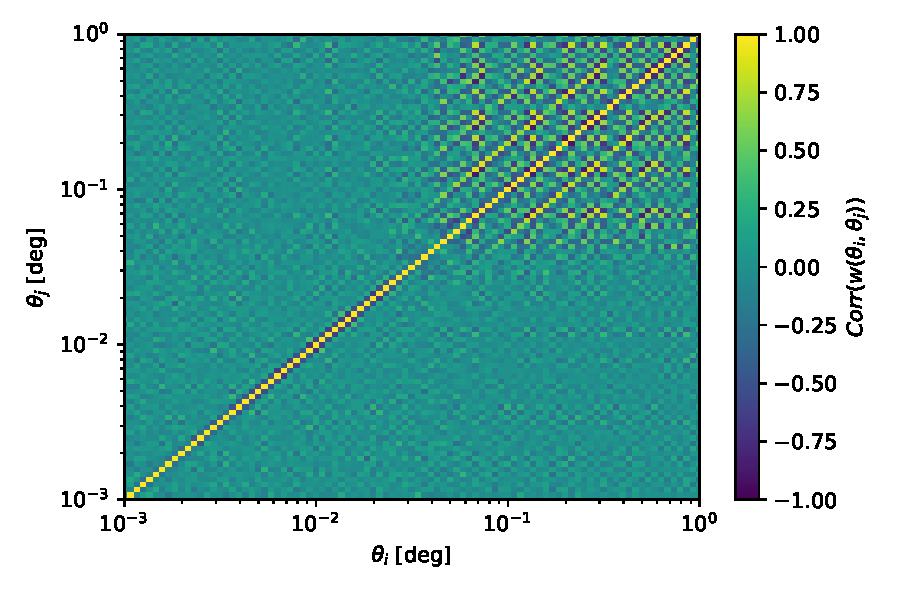
\includegraphics[width=0.9\columnwidth]{correlation_matrix_dithered_25p3_v2.pdf}
%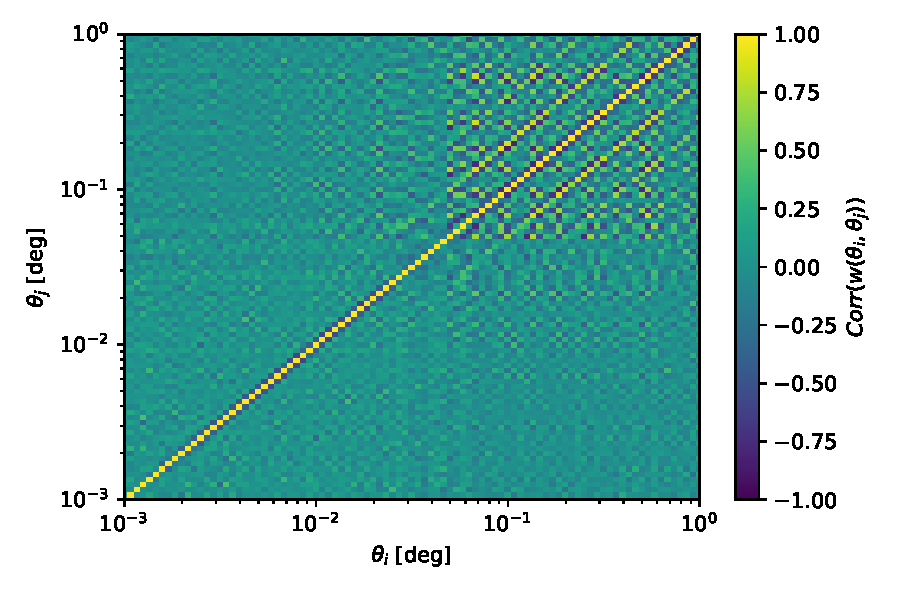
\includegraphics[width=0.9\columnwidth]{correlation_matrix_undithered_25p3_v2.pdf}
%\caption{Correlation matrices for the dithered (top) and undithered catalogs (bottom).}
%\label{fig:2pt_cov}
%\end{figure}
\subsubsection{Angular power spectrum}
We measure the angular power spectrum using the \texttt{NaMaster}\footnote{\url{https://github.com/damonge/NaMaster}} package~\citep{Namaster}. \texttt{NaMaster} computes the cross-power-spectra of spin-0 and spin-2 maps, with an arbitrary mask and number of contaminants using a pseudo-$C_{\ell}$ approach~\citep{2002ApJ...567....2H,2017MNRAS.465.1847E}. As we do for real space, we select the number of $\ell$-bins so that the covariance matrix is almost diagonal. In this case, we calculate the power spectrum in the range $0 < \ell < 6144$ and $\Delta \ell = 75$. We calculate the covariance matrices with three different approaches: The first approach is the same delete-one jackknife technique performed in real space; in the second approach, we compute the covariances using the mode-counting formula~\citep{Dodelson:1282338,2007MNRAS.381.1347C}
\begin{equation}
\mathrm{Cov}_{\ell\ell'}=\frac{2}{f_{sky}\Delta\ell}\left(\frac{C_{\ell}^{2}}{2\ell+1}+\frac{1}{\bar{n}^{2}}\right)\delta_{\ell\ell'}
\end{equation}
where $\bar{n}$ is the number density (objects per steradian). For the third approach we compute the Gaussian covariance with \texttt{NaMaster}. These three methods give consistent results. We compute the theoretical prediction for the power-spectra with \texttt{CCL}:
\begin{equation}
C_{\ell}^{TH} = \frac{2}{\pi}\int{dz} \left(\frac{dn(z)}{dz}\right)^{2} b^{2}(z) \int{dk k^{2} P(k,z)j^{2}_{\ell}(kr(z))}
\end{equation}
where $P(k,z)$ is the power spectrum, $b(z)$ is the bias and $\frac{dn}{dz}$ is the number density as a function of redshift. We use the Millenium cosmological parameters~\citep{2005Nature.435.629S} ($\Omega_{m}=0.25$,$\Omega_{b}=0.045$,$\Omega_{\Lambda}=0.75$, $n=1$, $\sigma_{8}=0.9$, $h=0.73$), and the $\frac{dn}{dz}$ built with the input catalog using the same magnitude cuts. The results are depicted in \figref{power_spectra}. We see that the results for both datasets follow the theoretical prediction within errors.
\begin{figure}
\centering
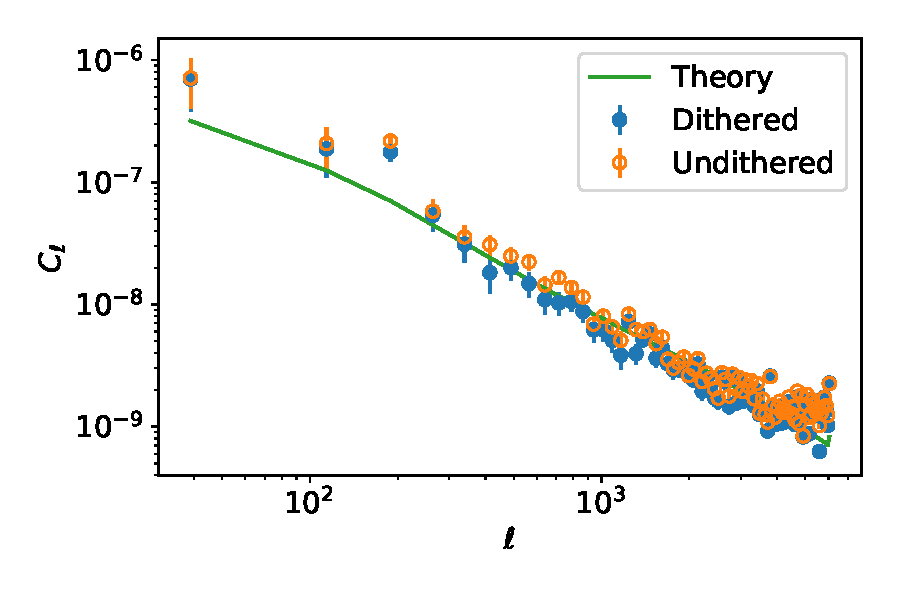
\includegraphics[width=0.9\columnwidth]{Cl_25p3_errors}
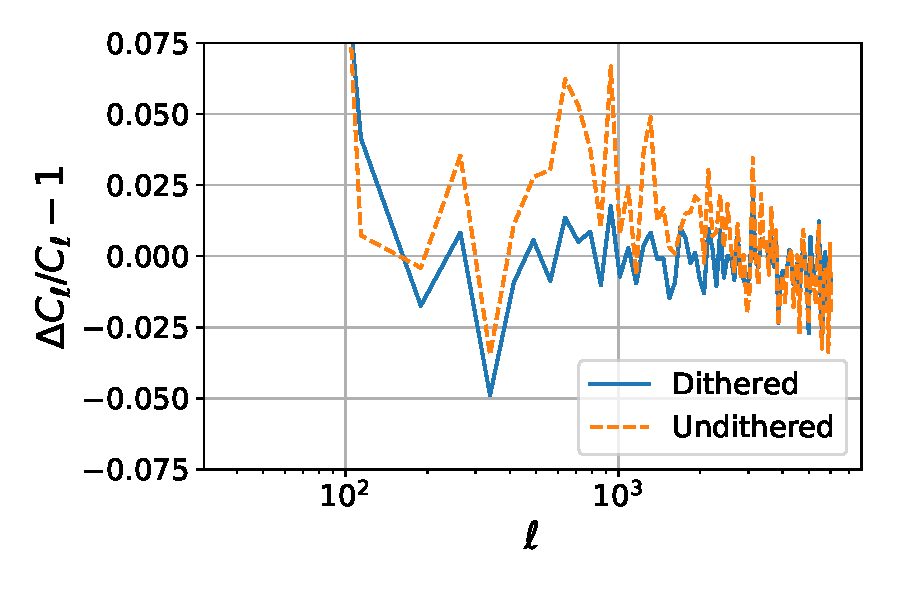
\includegraphics[width=0.9\columnwidth]{Cl_25p3_sys_comparison}
\caption{{\bf Top panel:} Measured power spectra undithered (open orange circles) and dithered (solid blue circles) datasets with \texttt{NaMaster} corrected by systematics. The error bars are computed using the Gaussian approximation. All datasets seem to be compatible with the theoretical prediction (green line) within 1-$\sigma$. {\bf Bottom panel:} Correction in harmonic space due to the different potential sources of systematic uncertainty relative to the value of the measured correlation function of the dithered (solid blue) and undithered (dashed orange) datasets}
\label{fig:power_spectra}
\end{figure}
\subsubsection{Systematic effects}
\label{ssec:systematics}
In this section, we analyze the different systematic effects affecting the DC1 data. We consider the following observational quantities as sources for systematic uncertainties:
\begin{itemize}
\item Extinction: The CatSim catalog provides the value for the magnitudes corrected for extinction using the map from \citet{1998ApJ...500..525S}. We will refer to as SFD map.
\item Stellar contamination: In this case, we build a HEALPix map using the input CatSim stellar catalog.
\item Sky-background: We use the observed background level in each exposure and assign that value to the HEALPixel with $N_{side}=2048$ that corresponds to the center of the field of view for each visit. After this we calculate the median value in each HEALPixel to build a map. The caveat of this approach is that we are not propagating the geometry of the focal plane.
\item Sky-noise: We use the observed noise background level in each exposure and proceed as in the previous case to build a HEALPix map with which we cross-correlate.
\item Seeing: We proceed as before and use the observed seeing in each exposure and build a HEALPix map.
\end{itemize}
These maps are shown in \figref{systematic_maps} and \figref{systematic_maps2}.

In the case of the real space measurements, we proceed as in \citet{2016MNRAS.455.4301C} to compute the impact of the different potential sources for systematic uncertainty. We compute the auto and cross-correlations of these maps and our data samples to obtain the ``true`` correlation function:
\begin{equation}
w^{gg}(\theta)_{true} =w^{gg}(\theta)_{obs} -  \vec{w}_{g,sys} \cdot W_{sys,sys}^{-1} \cdot \vec{w}_{g,sys}
\end{equation}
where $w^{gg}_{true}$ is the corrected galaxy-galaxy correlation function, $w^{gg}_{obs}$ is the measured galaxy-galaxy autocorrelation, $\vec{w}_{g,sys}$ is the vector containing the cross-correlation between the galaxies and the different maps, and $W_{sys,sys}^{-1}$ is the inverse of the matrix containing the cross-correlations between different systematics. For the stellar contamination, we also follow the procedure presented in~\citet{2016MNRAS.455.4301C}. Given a stellar fraction $f_{star}$, the ``true'' galaxy correlation function is given by
\begin{equation}
w_{gal} = \left(1+f_{star}\right)^{2}\left(w_{obs} - f_{star}^{2}w_{sg} - \frac{f_{star}^{4}}{\left(1+f_{star}\right)^{2}}\right)
\end{equation}
where $w_{sg}$ is the cross-correlation between our stellar map and the observed galaxies.

We select those objects classified as galaxies whose centroids lie within 2 pixels of a star from the input catalog and a measured magnitude within 30 mmags of that from the input star. By doing this, we estimate a stellar contamination of $f_{star}=7.2\%$ in our sample.

We compare the correction term, $\vec{w}_{g,sys} \cdot W_{sys,sys}^{-1} \cdot \vec{w}_{g,sys}$, for the different systematics to the measured signal obtaining the results in the middle and bottom panels of \figref{2pt_corr}. We show that the dither strategy works to reduce the impact of systematic effects at the percent level)for $\theta < 0.03$ degrees in this ``small`` area, improving the signal-to-noise. This is also seen at the top panel of \figref{2pt_corr}, where we clearly see that the uncorrected and corrected correlation function for the dithered field are essentially the same.

%\begin{figure}
%\centering
%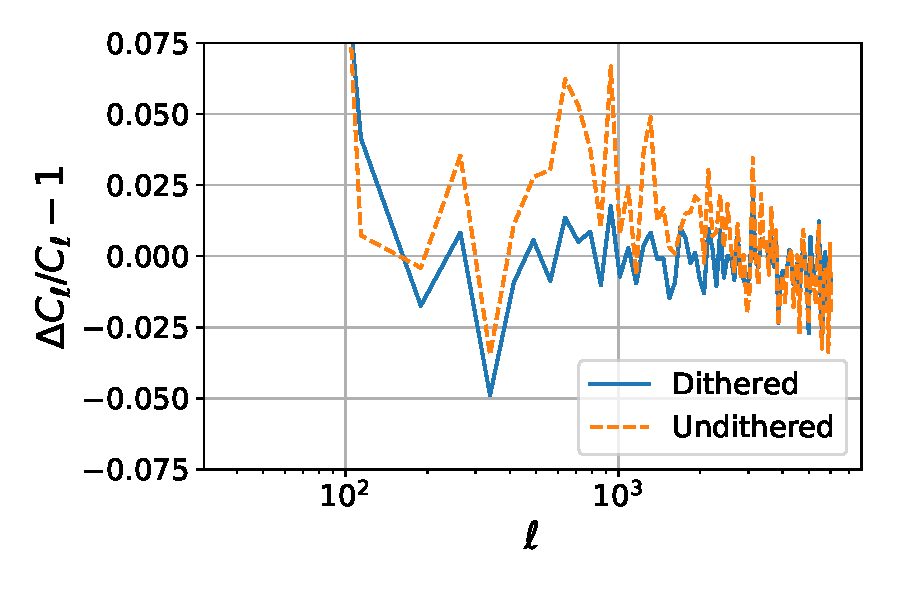
\includegraphics[width=0.9\columnwidth]{Cl_25p3_sys_comparison}
%\caption{Correction in harmonic space due to the different potential sources of systematic uncertainty relative to the value of the measured correlation function of the dithered (solid blue) and undithered (dashed orange) datasets.}
%\label{fig:sys_harmonic_space}
%\end{figure}


In the case of harmonic space, we use the mode deprojection from \texttt{NaMaster}~\citep{Namaster} to correct for the different templates. In the bottom panel of \figref{power_spectra}, we show the relative size of the correction due to the presence of the considered sources of systematic uncertainty. Again, we see that the dithered strategy diminishes the effect of the potential sources of systematic uncertainty in the power-spectrum measurements.

%\CHECK{Add figure with corrected and uncorrected power-spectra.}

%\subsection{Pushing the dataset further}

%We also wanted to check what happens if we choose a sample where the uniformity across the footprint is still good even though completeness is not as good. We extended our sample by selecting galaxies with \texttt{ $16 < $ CMODEL\_MAG $ < 26.25$} and depth$\geq 26.25$. This increases the sample from 4.3 million galaxies to 6.5 million in the dithered sample, even though the footprint is reduced by $8\%$. However, these selection criteria reduce the number of galaxies to 4.2 million in the undithered sample, as well as the footprint by $35\%$.

\subsection{Reconstructing the selection function}
As mentioned before, one of the potential applications of this kind of end-to-end studies is the possibility of analyzing how the pipeline performs data detection and measurement. In terms of the two-point statistics, we could think of this as a selection (window) function. In this section we are going to try to reconstruct the selection function given our input and output catalogs.

We use the spatial matching in \secref{matching} to get the magnitude and the error distribution for our detected galaxies. Then, we bin our sample in 100 true-magnitude bins from 18 to 28, and model the difference between input and output flux, $\Delta F$=$F_{meas}$-$F_{true}$, in each bin using a Gaussian mixture model (GMM) with 6 components for objects brighter than 26.4, and 3 components for fainter objects. We chose this threshold since it is close to our faintest $5\sigma$ limiting magnitude. This way, we have 100 models (one per magnitude bin) to distort the true magnitude and get a reconstructed (or emulated) magnitude. An example of this GMM is shown in \figref{example_GMM}. We see that, in a given bin, the GMM captures the overall distribution of $\Delta F$ well, allowing us to model the flux errors as a function of magnitude.
\begin{figure}
\centering
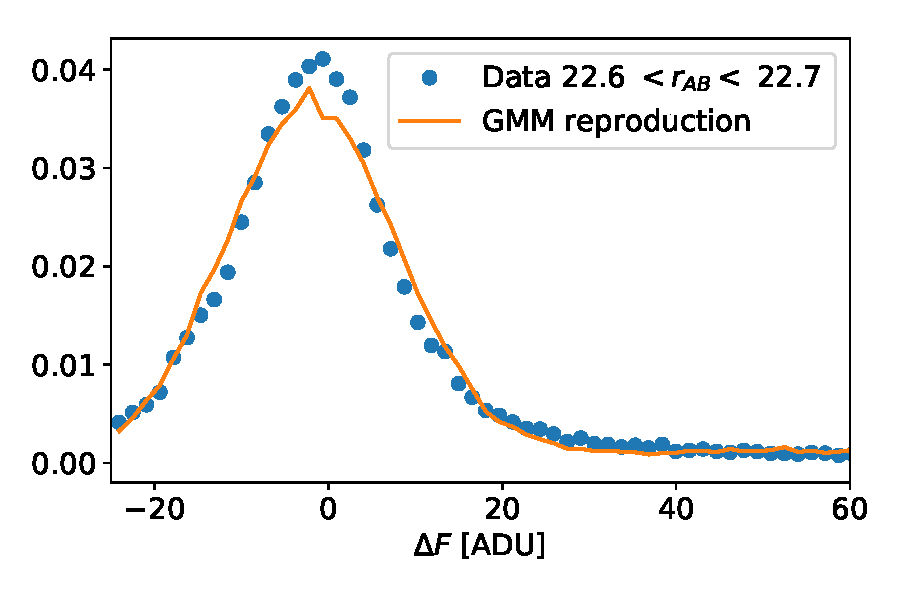
\includegraphics[width=0.9\columnwidth]{example_GMM}
\caption{Measured $\Delta F$ (blue solid circles) compared to 69,000 samples of the Gaussian mixture model that we obtain in the bin $22.6 <$ mag$_{true} < 22.7$. We repeated this for 100 bins between $18 <$ mag$_{true} < 28$.}
\label{fig:example_GMM}
\end{figure}

There are several caveats with this approach: $\Delta F$ is not Gaussian in the center of the distribution, which means that the GMM, regardless of its number of components, will show a slightly larger error than with real data. The second, bigger, caveat is that the models are constructed from detected objects but no information from the non-detected objects biasing the modeled $\Delta F$ is included. When we try to impose some cuts in our reconstructed magnitudes, we recover a larger number of objects than the detected number. This is shown in \figref{emulated_magnitudes}, where we use the emulated magnitudes to resemble the selection made in previous sections, i.e., including selected objects with $25.3 \geq r_{emulated} \geq 21.4$. We see that up to $r _{true} \approx 26$, we have a high level of completeness. We also see that our emulation, even though it gives us a larger number of detected objects, does a good job following the shape of the magnitude distribution. Above $r_{true}=26$, we are dominated by the outliers in the distribution of $\Delta F$ and we detect more objects than we should. We can also see that, if we only use objects such that $25.3 \geq r_{true} \geq 21.4$, we obtain a biased estimation of the two-point statistics, given that in this case we ignore the (heavy) tails of the magnitude distribution.
\begin{figure}
\centering
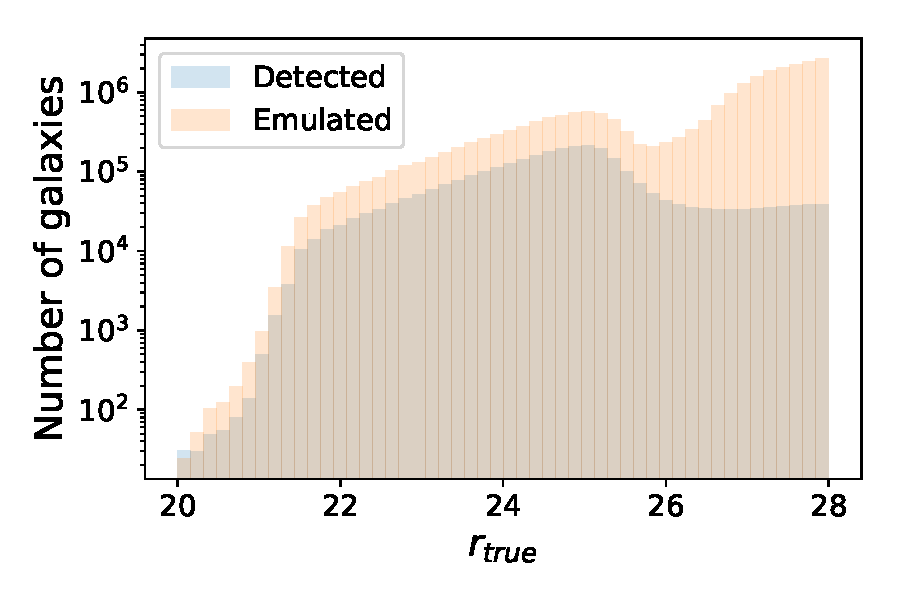
\includegraphics[width=0.9\columnwidth]{emulated_magnitude_histogram}
\caption{True magnitude distribution for the detected objects using spatial matching (blue) and for the emulated objects using the same cuts in measured and emulated magnitude, $25.3 \geq r \geq 21.4$}
\label{fig:emulated_magnitudes}
\end{figure}
In \figref{emulated_power} we show that the power-spectrum using the true magnitude cuts is very close to the power-spectrum of the detected objects. However, at small scales, it is smaller than the power-spectrum of the detected objects. This is likely due to the presence of fainter objects in the detected  sample. In addition, blended objects can create a small contribution at these scales. Finally, the larger shot-noise can make the residuals at small scales larger. On the other hand, at large scales, the power-spectrum using the true magnitude cuts is slightly larger due to the smaller magnitude range (and likely redshift range) considered. We also see that the power-spectrum for the emulated magnitude cuts is noticeably lower than the one for the detected objects. This is due to the larger magnitude range considered in the emulated sample (so we are averaging over a bigger volume in general). It is clear that this procedure is not good to emulate the selection function of our pipeline, given the sensitivity of LSST. We also see that performing cuts on the true magnitude distribution is not enough to recover the measured power-spectrum at the level of precision that we will have with LSST data. Therefore, more sophisticated ways of emulating the processing pipeline should be implemented, and tools like \texttt{BALROG}~\citep{2016MNRAS.457..786S}, \texttt{imSim}, or \texttt{PhoSim}~\citep{2015ApJS..218...14P} that generate synthetic images applied to random (zero-power-spectra) catalogs are interesting for future studies, in an effort to achieve percent-level sensitivities.
\begin{figure}
\centering
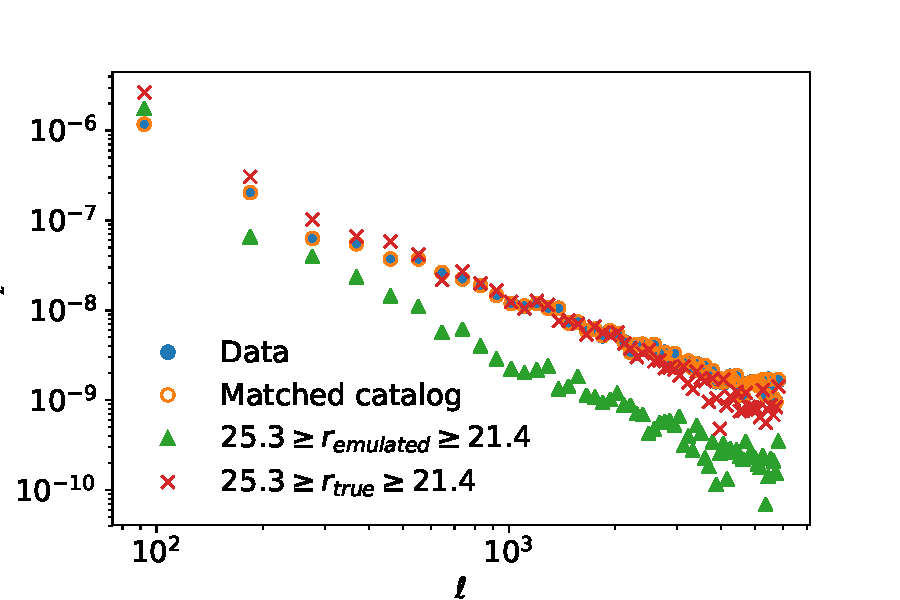
\includegraphics[width=0.9\columnwidth]{emulated_power_spectra}
\caption{Shot-noise subtracted measured power-spectra for the detected objects by the LSST tack (solid blue circles), the objects in the true catalog spatially matched (open orange circles), the objects with $21.4 \leq r_{true} \leq 25.3$ (red crosses), and the objects with $21.4 \leq r_{emulated} \leq 25.3$ (green triangles).}
\label{fig:emulated_power}
\end{figure}
% ----------------------------------------------------------------------

\section{Conclusions}
\label{sec:conclusions}

End-to-end simulations are very useful tools to test the overall performance of any current and future cosmological experiments like the LSST~\citep{Overview}. They allow us to test and improve different parts involved in the data processing and analysis, as well as, to model and improve our control of systematic uncertainties.

In this paper, we have presented a simulated (end-to-end) imaging dataset that resembles single-band, full-depth LSST data, for the first data challenge in the LSST DESC. We simulated images using state of the art tools (\textit{imSim}). We generated two different and complementary datasets, one with random dithers (\textit{dithered}) and the other with no dithers (\textit{undithered}). We processed these images with the LSST DM stack. We performed several quality assurance tests on the outputs from the DM stack, including photometry and astrometry checks. We checked that both the \textit{dithered} and \textit{undithered} are high-quality datasets with good photometry and astrometry (with the caveat of uncorrected proper motion).

We studied different ways to relate the output catalogs to the inputs. In particular, we studied two different matching strategies. The first, using information about positions only; and a second strategy involving positions and magnitudes. We showed that the angular power-spectrum is recovered at a very high-level of precision in both cases. However, these matching techniques are likely not good enough for studies about blending or very small scale information since they do not include information about undetected sources present in blends. An important research topic for these kind of end-to-end simulations is to find efficient strategies to relate inputs and outputs.

Finally, we estimated the depth of our simulated catalogs and selected a high-completeness sample to perform clustering analysis in both real and harmonic space. The results of this analysis, indicate that the simulated foregrounds have a low impact at the scales considered for our study, i.e. lower than $5\%$ for $\theta < 0.03^{\circ}$ (or for $100 < \ell < 6000$), especially in the \textit{dithered} dataset. This indicates the success of the dither strategy considered in this study. We also conducted a pilot study to try to reconstruct the selection function of our pipeline. We showed that simple methods cannot capture the complexity of our data given the high sensitivity that we will have in LSST and concluded that more complex methods should be studied in order to create better models.

The methodology presented in this work will serve as basis for future DESC data challenges, where we aim to perform multi-band studies in a larger area, analyze complementary image generation strategies (\texttt{PhoSim}), and increase the complexity of the foregrounds included.

% ----------------------------------------------------------------------

\subsection*{Acknowledgments}

This research used resources of the National Energy Research Scientific Computing Center, a DOE Office of Science User Facility supported by the Office of Science of the U.S. Department of Energy under Contract No. DE-AC02-05CH11231. We acknowledge the use of \texttt{Pandas, Dask, SciPy, Matplotlib, Jupyter, CCL, NaMaster, Healpy, and scikit-learn} as well as the LSST software stack.

The work of JC, RD, SD, TG, AJ, HK, PJM and BVK was supported by the U.S. Department of Energy under contract number DE-AC02-76SF00515.

%
The DESC acknowledges ongoing support from the Institut National de Physique Nucl\'eaire et de Physique des Particules in France; the Science \& Technology Facilities Council in the United Kingdom; and the Department of Energy, the National Science Foundation, and the LSST Corporation in the United States.  DESC uses resources of the IN2P3 Computing Center (CC-IN2P3--Lyon/Villeurbanne - France) funded by the Centre National de la Recherche Scientifique; the National Energy Research Scientific Computing Center, a DOE Office of Science User Facility supported by the Office of Science of the U.S.\ Department of Energy under Contract No.\ DE-AC02-05CH11231; STFC DiRAC HPC Facilities, funded by UK BIS National E-infrastructure capital grants; and the UK particle physics grid, supported by the GridPP Collaboration.  This work was performed in part under DOE Contract DE-AC02-76SF00515.
This manuscript has been authored by Fermi Research Alliance, LLC under Contract No. DE-AC02-07CH11359 with the U.S. Department of Energy, Office of Science, Office of High Energy Physics.

% 


%{\it Facilities:} \facility{LSST}

% Include both collaboration papers and external citations:
\bibliography{lsstdesc,main}

\appendix
\section{Mapping observational effects}
\label{sec:systematic_maps}
\begin{figure}
\centering
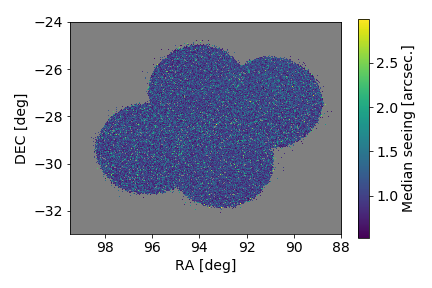
\includegraphics[width=0.7\columnwidth]{median_seeing.png}
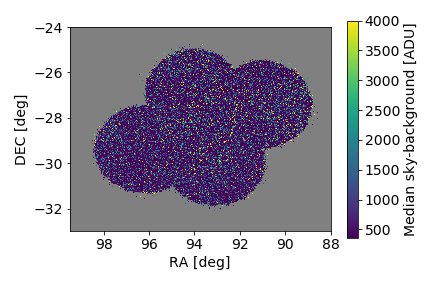
\includegraphics[width=0.7\columnwidth]{median_skybg.png}
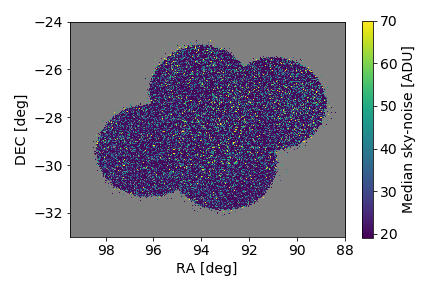
\includegraphics[width=0.7\columnwidth]{median_skynoise.png}
\caption{HEALPix maps showing the different observational effects that might be potential cause of systematic uncertanties.}
\label{fig:systematic_maps}
\end{figure}
\begin{figure}
\centering
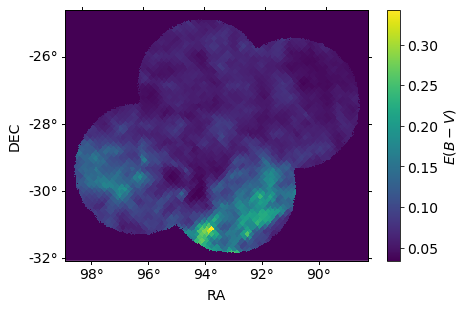
\includegraphics[width=0.7\columnwidth]{extinction.png}
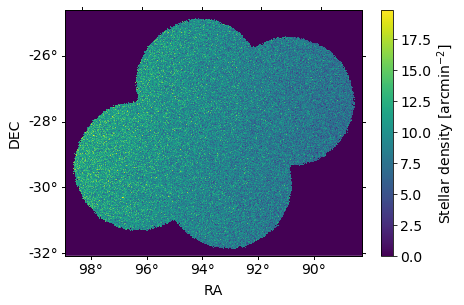
\includegraphics[width=0.7\columnwidth]{stellar_density.png}
\caption{HEALPix maps showing the different observational effects that might be potential cause of systematic uncertanties.}
\label{fig:systematic_maps2}
\end{figure}
%\section{Comparison of depth estimation methods}
%\begin{figure}
%\centering
%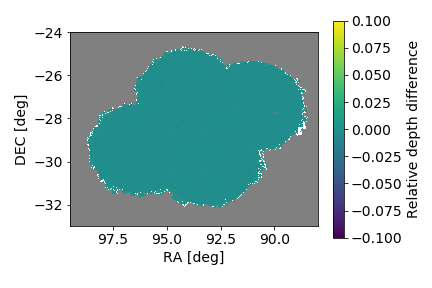
\includegraphics[width=0.9\columnwidth]{dithered_difference.png}
%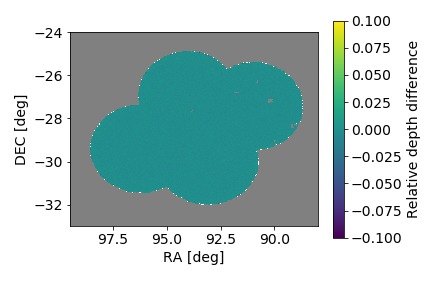
\includegraphics[width=0.9\columnwidth]{undithered_difference.png}
%\caption{Relative difference between the depth calculated using the two methods presented in the text for the dithered (top) and undithered (bottom) fields.}
%\label{fig:depth_comparison}
%\end{figure}
\end{document}


% ======================================================================
%
